\begin{comment}
\documentclass[11pt]{article}  % , titlepage
\usepackage{Common/toshi}
\begin{document}
\end{comment}


%%%%%%%%%%%%%%%%%% section 2 %%%%%%%%%%%%%%%%%%%%%%%%%%%%%%%%%
\section{Integrability from extra dimensions}
\label{sec:integrability}


Throughout this paper, we discuss correspondences between
a certain class of supersymmetric gauge theories and integrable lattice
models:
\begin{equation}
  \mathcal{I}_{\mathsf{T}_{4d}\left[\mathsf{L}_{2d}\right]}
    =  Z_{\mathsf{L}_{2d}\left[\mathsf{T}_{4d}\right]},
  \label{eq:correspondence}
\end{equation}
where the left-hand side is the supersymmetric index of a four-dimensional
gauge theory $\mathsf{T}_{4d}$ and the right-hand side denotes the
statistical partition function of the corresponding integrable lattice
model $\mathsf{L}_{2d}$ specified by the four-dimensional theory
$\mathsf{T}_{4d}$. As it turns out, the correspondence emerges from
TQFT with extra dimensions \cite{Yagi:2015lha}. The aim of this section is
to give the step-by-step explanation of the above correspondence from
an elementary level. Besides, to explain these, we will start by clarifying
the precise meaning of the terms TQFT, lattice model, and integrability.





\subsection{Preliminaries}

In section \ref{sec:lattice_model}, we will introduce lattice model as
discrete quantum field theory (QFT). So let us start from the general
settings of QFT. We first briefly review one-dimensional QFT, which
is nothing but quantum mechanics, and then extend the discussion to
general quantum field theory in $(d+1)$-dimensions. Though we do
not have a complete definition of general QFT, a special class of
QFT which is called \emph{topological} QFT is axiomatized by Atiyah
\cite{Atiyah:1989vu}.





\subsubsection{What is quantum field theory?}
\label{sec:what_is_qft}

Let us begin with one-dimensional QFT, as known as quantum mechanics
(QM). Suppose we have a one-dimensional manifold%
%
\footnote{Throughout the paper, we assume all the manifold is smooth and oriented,
unless otherwise stated. }%
%
, which may be thought of as ``time'' $M^{1}=$ interval or $S^{1}$
(or $\mathbb{R}$), and data to specify a QM:
\begin{itemize}
  \item $\mathcal{H}$ : a vector space (Hilbert space/state space),
  \item $\mathcal{O}$ : a set of self-adjoint operators (observables, acting on $\mathcal{H}$),
  \item $H$ : an operator called \emph{Hamiltonian},
\end{itemize}
where $H\in\mathcal{O}$, and the state space $\mathcal{H}$ is a finite
or an infinite dimensional $\mathbb{C}$-vector space. We sometimes need
to allow a set of operators $\mathcal{O}$ include not self-adjoint
operators, but for simplicity we do not care about that at this moment.
In undergraduate, we have learned that one should consider the Schr\"{o}dinger
equation and find a good basis in $\mathcal{H}$ which diagonalizes the
Hamiltonian.

As is well known, the procedure of solving the Schr\"{o}dinger equation, at least formally, leads
to an expression of time evolution of states by a linear map%
%
\footnote{We here do not get into the argument of Euclideanization.}
%
$e^{-tH}$ in quantum mechanics, and the partition function in many-body
statistical mechanics. In turn, we have two most crucial properties
of QM. Given an interval $M^{1}=\left[t_{0},t_{1}\right]$, we have
state vectors at the endpoints of the interval and a time evolution
between the states:
\begin{equation}
    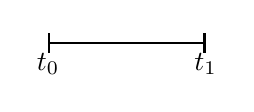
\begin{tikzpicture}[scale=1.0, baseline=(x.base)]    \node (x) at (0,0) {\vphantom{x}};

        \draw[thick, arrows=|-|] (0,0) node[below=0.1] {$t_0$} -- (2,0) node[below=0.1] {$t_1$};

    \end{tikzpicture}
  \quad \rightsquigarrow \quad
  e^{-(t_{1}-t_{0})H} : \mathcal{H}  \longrightarrow  \mathcal{H}
~ ,
\label{eq:qm_linearmap}
\end{equation}
and given a circle $M^{1}=S_{\beta}^{1}$, we get a number called
\emph{partition function}:
\begin{equation}
    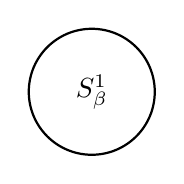
\begin{tikzpicture}[scale=0.8, baseline=(x.base)]    \node (x) at (0,0) {\vphantom{x}};

        \draw[thick] (0,0) circle[radius=1cm] node {$S^1_{\beta}$};
%        \draw[thick] (0.9,0) -- (1.1,0) node[right] {$t=0,\, \beta$};
%        \node at (0.5,1.5) {\large${\rm Tr}_{\mathcal{H}} e^{-\beta H}$};

    \end{tikzpicture}
  \quad \rightsquigarrow \quad
  \mathrm{Tr}_{\mathcal{H}}  e^{-\beta H}
~ .
\label{eq:qm_number}
\end{equation}


%FIGURE
\begin{figure}
\centering
  \subfloat[\label{}]{  % fig:qm_interval
    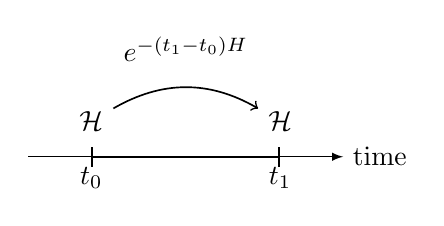
\begin{tikzpicture}[scale=1.0] %, baseline=(x.base)]    \node (x) at (0,0) {\vphantom{x}};

        \draw[arrows=-latex] (0,0) -- (4,0) node[right] {time};
        \draw[thick, arrows=|-|] (0.8,0) node[above=0.2cm] (H0) {\normalsize $\mathcal{H}$} node[below=0.1] {$t_0$} -- (3.2,0) node[above=0.2cm] (H1) {\normalsize $\mathcal{H}$} node[below=0.1] {$t_1$};
        \draw[semithick, arrows=-to] (H0) to[bend left=30] node[above=0.2cm, pos=0.5] {\normalsize $e^{-(t_1 - t_0)H}$} (H1);

    \end{tikzpicture}
  }
  \qquad\qquad
  \subfloat[\label{}]{  % fig:qm_circle
    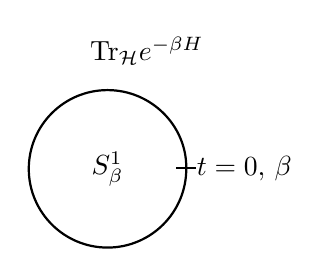
\begin{tikzpicture}[scale=1.0] %, baseline=(x.base)]    \node (x) at (0,0) {\vphantom{x}};

        \draw[thick, arrows=|-] (1,0) node[right=0.1] {$t=0,\, \beta$} arc (0:360:1);
        \node at (0,0) {$S^1_{\beta}$};  %\normalsize

%        \draw[thick] (0,0) circle[radius=1cm];
%        \draw[thick] (0.9,0) -- (1.1,0) node[right] {$t=0,\, \beta$};
        \node at (0.5,1.5) {\normalsize ${\rm Tr}_{\mathcal{H}} e^{-\beta H}$};

    \end{tikzpicture}
  }
  \caption{Two most crucial properties of quantum mechanics.}
  \label{fig:qm_two_properties}
\end{figure}


In addition, from physical facts it is quite reasonable to assume
that the time evolution and the partition function are compatible
with cutting and gluing intervals and $S^{1}$s. This simply means
that a time evolution from time $t_{0}$ to $t_{1}$ followed by
another time evolution from $t_{1}$ to $t_{2}$ is equal to a single
time evolution from $t_{0}$ to $t_{2}$, etc. Summarizing, the properties
of quantum mechanics, or one-dimensional QFT, are rephrased by
the language of given one-dimensional manifold $M^{1}$ (see figure \ref{fig:qm_two_properties}):
\begin{itemize}
  \item Given an interval, QM produces state vectors at the endpoints and a linear
map between them.
  \item Given an $S^{1}$, QM produces a number.
  \item These two properties are compatible with cutting and gluing intervals and $S^{1}$s.
\end{itemize}
Thus, in the abstract we conclude that quantum
mechanics is a gadget satisfying the above properties for each given
one-dimensional manifold $M^{1}$.

From these observations of quantum mechanics, we wish to extend the
discussion to general $(d+1)$-dimensional QFT. The starting point
of defining a $(d+1)$-dimensional QFT is the choice of a $(d+1)$-dimensional
manifold $M^{d+1}$, which has $d$ spatial directions and one ``time''
direction. For most QFTs the manifold $M^{d+1}$ is viewed as a Riemannian
manifold with a smooth metric on it. As already noticed, we will mostly
consider a positive definite Riemannian metric, QFT on which is usually
referred to as an Euclidean QFT, and hence precisely there is no notion
of ``time'' in such a theory, at least globally. The manifold $M^{d+1}$
may or may not have boundaries. In case it does have boundaries some
additional information is needed at the boundaries to define the QFT.
In addition to a Riemannian metric, depending on the situation one
wants to consider, one often needs some more structures on the manifold
$M^{d+1}$, e.g. smooth structure, conformal structure, spin structure,
etc.

To obtain the data to specify a QFT, we now would like to extend the
observations seen in QM. Suppose we have a $(d+1)$-dimensional manifold
$M^{d+1}$, then we wish to ``define'' a QFT by a gadget $Z$, which
should produce a vector when $M^{d+1}$ has a boundary
\begin{equation}
Z\big(M^{d+1}\big)  \in  \mathcal{H}_{bdy},
\end{equation}
and should produce a number when $M^{d+1}$ has no boundary
\begin{equation}
Z\big(M^{d+1}\big)  \in  \mathbb{C}.
\end{equation}
In the case of $M^{d+1}$ with a boundary, the vector space associated
on the boundary is called the space of states or just Hilbert space
in the physics literature. On the one hand, if $M^{d+1}$ does not
have boundary, the number $Z\big(M^{d+1}\big)$ is called the partition
function. When the boundary of $M^{d+1}$ consists of several disconnected components,
namely the boundary is given by a disjoint union of simply connected
$d$-dimensional closed manifolds $\big\{ N_{i}^{d}\big\}$: $\partial M^{d+1}=\sqcup_{i}N_{i}^{d}$,
$Z$ should define a linear map among the vector spaces defined on
the boundaries. In particular, in the case $M^{d+1}=N^{d}\times I$,
where $I$ is an interval of length $T$, $M^{d+1}$ has two boundaries
$N^{d}$ and $Z$ now gives rise to a linear map $Z\big(N^{d}\times I\big)=:U(T)$,
\begin{equation}
  U(T) : \mathcal{H}_{N} \longrightarrow \mathcal{H}_{N}.
\end{equation}
From  physical facts, $Z$ also should be compatible with cutting and
gluing of $(d+1)$-dimensional manifolds, and thus we learn that the
linear map given above satisfies $U(T_{1})U(T_{2})$ $=$ $U(T_{1}+T_{2})$.
This really defines an operator $H$ as the generator of $U$,
\begin{equation}
  U(T)  =  \exp (-TH).
\end{equation}
$H$ is called the Hamiltonian of the system, acting on the space
of states $\mathcal{H}_{N}$. If one considers a manifold
with Lorentzian metric, $U(T)$ is represented as
\begin{equation}
  U(T)  =  \exp (-iTH),
\end{equation}
and then the interval $I$ is regarded as ``physical time.''





\subsubsection{Construction of $Z$}

So far we have discussed only in an abstract way what quantum field
theory is, or in other words what the gadget $Z$ should satisfy.
Let us now see how we specify $Z$ to define a QFT. Broadly speaking,
there are three kinds of constructions of $Z$. They are not totally
independent and have many aspects of applicabilities. In the rest
of this section, $M$ denotes a $(d+1)$-dimensional manifold with
or without boundary, and $N$ denotes a $d$-dimensional closed manifold
without boundary.

\subsubsection*{Construct from an axiom}

The first construction is in a sense the simplest one; we write down
appropriate properties that a QFT must satisfy, and axiomatize them.
Construction of $Z$ is to give a mathematical formulation which satisfies
the axioms as the data to specify the theory. This is actually the
only way that one can define a QFT by mathematically rigorous procedures.
Normally, such a theory is first studied by physicists as an ideal
or a toy model from physical motivations, and then refined as rigorous
mathematics by mathematicians.%
%
\footnote{The fact that a QFT can be treated in a mathematically rigorous way
implies that the theory may have an enormous amount of symmetry, and
the difficulties of the QFT are completely controlled by them. Even
better, these theories can often be exactly solved in an appropriate
sense.}
%
There are several kinds of such theories. We now introduce typical
three examples.

The first one is \emph{free theories} in any dimensions, which are
toy models of field theories and play important roles as a probe of
more complicated QFTs. In any spacetime dimensions, for the Riemannian
manifolds with or without spin structure, we can rigorously define
the free field theories. One of them is the free scalar field theory.
Besides a $(d+1)$-dimensional closed manifold $M$, pick a $G$-bundle
$P\to M$ with a connection $A$ and a $G$-vector space $V$.
Then we construct the associated vector bundle $P\times_{G}V$, whose
covariant derivative is denoted by $D_{A}$. We now have the Laplacian
$\Delta_{A}$ given by the covariant derivative $D_{A}$, and then
the free scalar field theory is defined by the partition function
\begin{equation}
  Z_{\mathrm{scalar}}(M;A)  :=  1/\det\Delta_{A}.
\end{equation}
If the determinant of the Laplacian involves a divergence, it must
be properly regularized.

Another free theory is the free fermion theory. In this case $M$
also needs a spin structure and the spin representations $S$, $S'$.
Then we construct the Dirac operator $\mathcal{D}_{A}$ on the spin
bundles, and the partition function of the free fermion theory is given
by
\begin{equation}
Z_{\mathrm{fermion}}(M;A):=\det\mathcal{D}_{A},
\end{equation}
again the determinant is taken appropriately.%
%
\footnote{Fermion theories may have anomalies. If it is the case, the axiom
needs to be somehow modified. In particular the partition function
for a closed manifold is given by the eta invariant \cite{Dai:1994kq}.}

Next, in two dimensions, we have another axiomatic quantum field theory,
that is \emph{conformal field theory} (CFT).
To discuss two-dimensional CFT, we need a conformal (complex) structure
on $M$, i.e. $M$ becomes a Riemann surface. CFT in two dimensions was formulated by Belavin, Polyakov,
and Zamolodchikov \cite{Belavin:1984vu} as a model of physical systems at critical
points. They established the renowned Virasoro algebra as an infinite
dimensional symmetry of the system and fully investigated the minimal
model. The holomorphic part of the Virasoro algebra is captured by
vertex operator algebras, and since then there are many mathematically
rigorous discussions on them. Their kinematic behaviors on Riemann
surfaces are governed by the conformal blocks, and its geometric meaning
has been studied in \cite{Friedan:1986ua}. In turn, the study of irrational
CFTs has led to the AGT correspondence \cite{Alday:2009aq}, which has brought
to us large amount of developments in both physics and mathematics.
We will give a general statement of AGT correspondence and apply it to our work
in section \ref{sec:line_defects}.

The final example is \emph{topological quantum field theories} (TQFTs).
TQFT is one of the main focuses in this paper. These theories
originate from Witten's proposals of topological field theories
\cite{Witten:1988xj, Witten:1988ze, Witten:1988hf}. Inspired by Witten's
works, Atiyah and Segal axiomatized the topological QFT,%
%
\footnote{Precisely speaking, what Segal axiomatized is the definition of conformal
field theories \cite{Segal:2002ei}. Segal's definition of CFT is categorical
and quite similar to the definition of Atiyah's TQFT.
For the geometric definition of CFT, see \cite{Friedan:1986ua}. }
%
and happily this also has brought to us a numerous amount of applications
both to physics and to pure mathematics. For example, ($1+1$)-dimensional
topological QFTs are known to be functorially equivalent to the category of commutative
<<<<<<< HEAD
Frobenius algebras \cite{MR2037238}. $(2+1)$-dimensional Chern-Simons theory for a
=======
Frobenius algebras. $(2+1)$-dimensional Chern-Simons theory for a
>>>>>>> dissertation
compact Lie group $G$ is rigorously constructed by Kohno \cite{MR1167165} using
the monodromy representation of Knizhnik-Zamolodchikov equation \cite{Knizhnik:1984nr},
and Turaev-Viro, Reshetikhin-Turaev using quantum groups \cite{Turaev:1992hq, Reshetikhin:1991tc}.
$(2+1)$-dimensional Chern-Simons theory has many
applications to knot or link invariants and $3$-manifold invariants.
Moreover, both 2d and 3d TQFTs have applications to the mirror symmetry,
or topological string theory (see e.g. \cite{Hori:2003ic}), those have led to fruitful interactions
between physics and mathematics. We will take more time for TQFT and
introduce the Atiyah's axioms in some detail in section \ref{sec:Atiyah_TQFT}.

\subsubsection*{Path integrate a Boltzmann weight}

Before going to Atiyah's TQFT axioms, let us see two more constructions
of $Z$. These are no longer mathematically rigorous, but rather familiar
constructions for physicists. The second construction is to define
a partition function by \emph{path integral}. The general prescription
is given as follows: One first introduces an action functional over
the classical field configurations, which deduces the classical equation
of motion by the variational principle. Then one exponentiates the
action and integrate it over the space of fields.

The partition function for the free fields given above can also be
defined by the path integral expression. For example, for the free
complex scalar field theory consider a section $\phi$ of the vector
bundle $P\times_{G}V$ over $M$, where $V$ is a representation of
a compact Lie group $G$. Then define an action functional

\begin{equation}
  S  :  \Gamma(P\times_{G}V)  \longrightarrow  \mathbb{R},
\end{equation}
such that
\begin{equation}
  S(\phi)  =  \int_{M}\frac{1}{2}D_{A}\phi\wedge\ast D_{A}\phi,
\end{equation}
where $*$ is the Hodge star on $M$. $D_{A}$ is again the covariant
derivative given by the connection $A$. Using this action functional,
physicists ``define'' its partition function by
\begin{equation}
Z_{\mathrm{scalar}}(M;A):=\int_{\Gamma(P\times_{G}V)}\mathcal{D}\phi\,e^{-S(\phi)}.
\end{equation}
The integrand $e^{-S}$ of path integral is generically called the
\emph{Boltzmann weight}. For the free field theories, the path integral
can be expressed as an infinite product of the Gaussian integral.
Introducing an appropriate regularization, one can compute the exact
partition function and it leads to the same result as mentioned above.

As another example, let us consider pure Yang-Mills theory. We introduce
the kinetic term of the connection $A$, and define the action functional
\begin{equation}
  S(A)  =  \int_{M}\frac{1}{4g^{2}}F_{A}\wedge*F_{A},
\end{equation}
where $F_{A}$ is the curvature of the $G$-connection $A$. Define
the partition function of Yang-Mills theory by
\begin{equation}
  Z_{\mathrm{YM}}(M)  =  \int_{\mathcal{A}_{M}/\mathcal{G}}\mathcal{D}A\,e^{-S(A)},
\end{equation}
where the integral is taken over the space of connections on $M$
modulo gauge transformations. Unlike the free scalar theory, making
this path integral mathematically precise is extremely difficult.
Although it is still ill-defined, physicists have been working
on this expression to understand many properties of quantum gauge
theories. Experimentally, we discretize the manifold $M$
to a $(d+1)$-dimensional lattice and put it on a supercomputer. At
least, numerical calculations show the above construction may be a
mathematically meaningful and reproduce many experimental results
to reasonable accuracy.

\subsubsection*{Deduce from string/M-theory}

The final construction of $Z$ is to use string or M-theory. This
is also our main tool to construct a QFT to realize the correspondence
\eqref{eq:correspondence}. Nonetheless, string or M-theory
is less rigorous than path-integral expression of the construction
of $Z$, and thus it is more hopeless to give a mathematically precise
meaning to the construction. We here would like to show just two examples
which ``define'' a class of quantum field theories through string/M-theory.

The first example is the AdS/CFT correspondence.

The second example is the so-called six-dimensional $\mathcal{N}=(2,0)$
superconformal field theories (SCFT) \cite{Witten:1995zh}. We start from a 10-dimensional string theory called the
type IIB string theory, which roughly speaking assigns the partition
function $Z_{\mathrm{IIB}}(\tilde{M})$ to a 10-dimensional
manifold $\tilde{M}$. Pick a finite subgroup $\Gamma_{G}$ of $\SU(2)$
of type $G=A_{n},\,D_{n}$ or $E_{6,7,8}$. We define a six-dimensional
QFT $Q_{G}$ by its partition function for a six-dimensional manifold
$M$,
\begin{equation}
Z_{Q_{G}}(M)  =  Z_{\mathrm{IIB}}\big(M\times\mathbb{C}^{2}/\Gamma_{G}\big).
\end{equation}
 They are examples of six-dimensional $\mathcal{N}=(2,0)$
superconformal QFTs. These theories are known not to have a Lagrangian
description, and hence their partition function cannot be obtained from
the path integral formulation. They have another description via M-theory,
as the low-energy dynamics of M5-branes. The construction from M5-branes
leads to the AGT correspondence and the notion of class-$\mathcal{S}$
theories, which we will explain in later sections.






\subsubsection{Atiyah's topological QFT}
\label{sec:Atiyah_TQFT}

As mentioned some times, in this paper TQFT in extra dimensions
plays a crucial role to realize the correspondence between supersymmetric
gauge theories and integrable lattice models. So now let us pause
here and introduce the Atiyah's axioms of TQFT \cite{Atiyah:1989vu}. We first list the
axioms, and right then give their physical meanings. Readers will
notice that most of these axioms are physically quite natural and
actually mathematical rephrasing of the properties that $Z$ should
satisfy, which we have already seen. In addition, we would like to
define lattice model as a discrete version of QFT in the next subsection.
Reviewing the definition of TQFT here will be a good help
of the argument of lattice model.


\subsubsection*{Axiom (Atiyah's ($d+1$)-dimensional TQFT)}

($d+1$)-dimensional TQFT is defined by $Z$ consisting of the following
two data and five assignments:
\begin{itemize}
  \item For each oriented $d$-dimensional closed manifold $N$, $Z$ assigns a
finite dimensional $\mathbb{C}$-vector space $\mathcal{H}_{N}$:
\begin{equation}
  Z(N)  =  \mathcal{H}_{N}.
\end{equation}
\end{itemize}
This corresponds to (a half of) canonical quantization, or geometric
quantization, known in physics literature. Why we say it is ``a half
of'' will be explained in a moment. In physics, especially for a
field theory which has a Lagrangian description, we consider the phase
space of fields, take a constant-time surface, and then perform canonical
quantization by imposing canonical commutation relations on fields
and their conjugate momenta. The constant-time surface is a codimension-1
hypersurface in $(d+1)$-dimensional manifold $M$, which in this
case is nothing but the $d$-dimensional closed manifold $N$. So,
the manifold $N$ is viewed as a collection of $d$ spatial directions.
One can think of the assigned vector space $\mathcal{H}_{N}$ as ``the
space of functionals on the classical fields on $N$,'' usually called
the space of states or just Hilbert space of the system. The only
major difference here is that for topological theory the Hilbert space
is of finite dimension.%
%
\footnote{One can remove the finiteness condition from the axiom. In
TQFT we can in fact define a non-degenerate bilinear form from the other axioms,
and from that as a corollary we can deduce the space of states is
finite-dimensional. }
%
\begin{itemize}
  \item For each oriented $(d+1)$-dimensional manifold $M$ with a boundary
$\partial M=N$, $Z$ assigns a vector
\begin{equation}
  Z(M)
  =
  Z\left(
    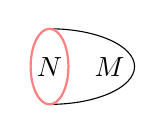
\begin{tikzpicture}[scale=0.6, baseline=(x.base)]    \node (x) at (0,0) {\vphantom{x}};
        \def\bdyradius{0.8cm}

        \draw (0,-\bdyradius) arc[start angle=-90,end angle=90,x radius=1.8cm,y radius=\bdyradius] node[left=0.1,pos=0.5] {$M$};
        \draw[thick, red!50] (0,0) node[black] {$N$} circle[x radius=0.4cm,y radius=\bdyradius];

    \end{tikzpicture}
  \right)
  \in  \mathcal{H}_{N}.
\end{equation}
\end{itemize}
This expresses the path integral quantization on $M$ with boundary.
Recall that if one has a spacetime manifold with boundary, one needs
to impose a boundary condition on fields on the boundary, and it leads
to the state vector associated to the boundary condition by path integral
expression; let $\varphi$ be a fixed field configuration on
$N$,
\begin{equation}
  Z(M;\varphi)  =  \int_{X\mid_{N}=\varphi}\mathcal{D}X \, e^{-S(X)} \,  \in  \mathcal{H}_{N}.
\end{equation}
 In other words, the quantum state at a generic time $t$ is given
by the path integral of the Boltzmann weight over all the classical
fields with time $<t$.


%FIGURE
\begin{figure}
\centering
  \subfloat[\label{}]{  % fig:one_bdy
    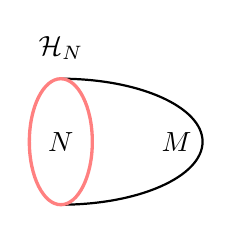
\begin{tikzpicture}[scale=1] %, baseline=(x.base)]    \node (x) at (0,0) {\vphanton{x}};
        \def\bdyradius{0.8cm}

        \draw[thick] (0,-\bdyradius) arc[start angle=-90,end angle=90,x radius=1.8cm,y radius=\bdyradius] node[left=0.3,pos=0.5] {$M$};
        \draw[very thick, red!50] (0,0) node[black] {$N$} circle[x radius=0.4cm,y radius=\bdyradius] node[above=\bdyradius+0.1cm, black] {\normalsize$\mathcal{H}_N$};

    \end{tikzpicture}
  }
\qquad\qquad
  \subfloat[\label{}]{  % fig:two_bdy
    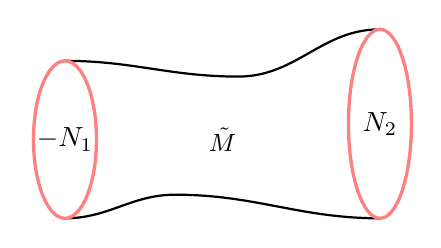
\begin{tikzpicture}[scale=1] %, baseline=(x.base)]    \node (x) at (0,0) {\vphanton{x}};
        \def\bdyradius{1cm}

        \draw[thick] (0,-\bdyradius) to[out=0,in=180] (1.4cm,0.3cm-\bdyradius) to[out=0,in=180] (4cm,0.2cm-\bdyradius*1.2);
        \draw[thick] (0,\bdyradius) to[out=0,in=180] (2.2cm,-0.2cm+\bdyradius) to[out=0,in=180] (4cm,0.2cm+\bdyradius*1.2);

        \draw[very thick, red!50] (0,0) node[black] {$-N_1$} circle[x radius=0.4cm,y radius=\bdyradius];
        \draw[very thick, red!50] (4,0.2) node[black] {$N_2$} circle[x radius=0.4cm,y radius=\bdyradius*1.2];

        \node at (2,0) {\small$\tilde M$};

    \end{tikzpicture}
  }
  \caption{$(d+1)$-dimensional manifolds $M$ and $\tilde{M}$.
  They have a single boundary and two disconnected boundaries.
  For each case, $Z$ gives a vector and a linear map, respectively.}
  \label{fig:mfd_w_bdys}
\end{figure}


These data are subject to the following assignments:
\begin{enumerate}
  \item (involutory) Let $-N$ denote a manifold $N$ with the opposite orientation,
then
\begin{equation}
  \mathcal{H}_{-N}  =  \mathcal{H}_{N}^{*},
\end{equation}
where $\mathcal{H}_{N}^{*}$ is the dual to $\mathcal{H}_{N}$.
  \item (multiplicative) If $N$ is a disjoint union of two $d$-dimensional
closed manifolds $N_{1}$ and $N_{2}$, then the vector space associated
on it is factorized to a tensor product:
\begin{equation}
  \mathcal{H}_{N_{1}\sqcup N_{2}}  =  \mathcal{H}_{N_{1}}  \otimes  \mathcal{H}_{N_{2}}.
\end{equation}
This is really natural in the physical point of view. This condition
means that if we have two physical systems defined on spatially disjoint
union $N_{1}\sqcup N_{2}$, then the space of states is represented
as the tensor product of each state space. Also, from the conditions
so far one finds that if a ($d+1$)-dimensional manifold $M'$ has two
boundaries such that
\begin{equation}
  \partial M'  =  -N_{1}\sqcup N_{2},
\end{equation}
then $Z$ defines a linear map
\begin{equation}
  Z\big(M'\big)
  =
  Z\left(
    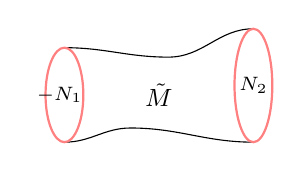
\begin{tikzpicture}[scale=0.6, baseline=(x.base)]    \node (x) at (0,0) {\vphantom{x}};
        \def\bdyradius{1cm}

        \draw (0,-\bdyradius) to[out=0,in=180] (1.4cm,0.3cm-\bdyradius) to[out=0,in=180] (4cm,0.2cm-\bdyradius*1.2);
        \draw (0,\bdyradius) to[out=0,in=180] (2.2cm,-0.2cm+\bdyradius) to[out=0,in=180] (4cm,0.2cm+\bdyradius*1.2);

        \draw[thick, red!50] (0,0) circle[x radius=0.4cm,y radius=\bdyradius];\node[black] at (-0.1,0) {\scriptsize $-N_1$};
        \draw[thick, red!50] (4,0.2) node[black] {\scriptsize $N_2$} circle[x radius=0.4cm,y radius=\bdyradius*1.2];

        \node at (2,0) {\small$\tilde M$};

    \end{tikzpicture}
  \right)
  \in  \mathrm{Hom}_{\mathbb{C}}\left(\mathcal{H}_{N_{1}},\mathcal{H}_{N_{2}}\right),
\end{equation}
namely, for a cobordism between $N_{1}$ and $N_{2}$, we have a
linear map between $\mathcal{H}_{N_{1}}$ and $\mathcal{H}_{N_{2}}$.
This defines a time evolution, or transition amplitude, between the
states in $\mathcal{H}_{N_{1}}$ and $\mathcal{H}_{N_{2}}$. When
the field theory has a Hamiltonian, $Z\big(M'\big)$ may correspond
to the time evolution operator
\begin{equation}
  Z\big(M'\big) := e^{-tH} : \mathcal{H}_{N_{1}} \longrightarrow \mathcal{H}_{N_{2}}.
\end{equation}
Since canonical quantization is a procedure to make an assignment
of Hilbert spaces and the time evolution on them, as we saw in QM,
this association of linear maps gives the other half of canonical
quantization.
One can also explicitly express $Z\big(M'\big)$ in the path integral
expression by the Feynman kernel (also as known as propagator or Green's
function). Suppose we have an initial state $\Psi_{0}\in\mathcal{H}_{N_{1}}$,
then the state $\Psi_{t}\in\mathcal{H}_{N_{2}}$ at time $t$ is expressed
by
\begin{align}
  \Psi_{t}(\varphi_{t})
  & =\left(e^{-tH}\Psi_{0}\right)  (\varphi_{t})  \nonumber \\
  & =\int K(\varphi_{t},\varphi_{0})\Psi_{0}(\varphi_{0})\mathcal{D}\varphi_{0},
\end{align}
where
\begin{equation}
  K(\varphi_{t},\varphi_{0})
    =\int_{X\mid_{N_{1}}=\varphi_{0}}^{X\mid_{N_{2}}
    =\varphi_{t}}\mathcal{D}X\,e^{-S(X)}.
\end{equation}
  \item For two cobordisms
\begin{equation}
  \partial M_1 =  -N_{1}\sqcup N_{2},  \quad  \partial M_2  =  -N_{2}\sqcup N_{3},
\end{equation}
it follows that
\begin{equation}
  Z\big(M_1  \cup_{N_{2}} M_2 \big)  =  Z(M_2)Z (M_1),
\end{equation}
where the cobordisms $M_1$ and $M_2$ are glued along $N_{2}$ by a
certain diffeomorphism on $N_{2}$. This asserts that the linear maps
are transitive when we compose cobordisms. This is nothing but the
physical requirement that the time evolution is compatible with the
cutting and gluing the manifolds.
  \item Given $N=\emptyset$ as an empty $d$-dimensional manifold, then the
associated vector space is one-dimensional:
\begin{equation}
  Z(\emptyset)  =  \mathbb{C}.
\end{equation}
This is a non-triviality condition. From this condition, for each $(d+1)$-dimensional
manifold $M$ without boundary, $\partial M=\emptyset$, $Z$ assigns
a number:
\begin{equation}
  Z(M)  \in  \mathbb{C}.
\end{equation}
This number associated to a closed $(d+1)$-dimensional manifold
is known as partition function. Not only is it an important quantity
physically, but it also has mathematical applications, such as giving
a topological invariant of the closed manifold $M$.
\item Let $I$ be an interval, then for each cylinder $M=N\times I$, the
linear map on $\mathcal{H}_{N}$ is trivial:
\begin{equation}
  Z(N\times I)  =  \mathrm{id}_{\mathcal{H}_{N}}.
\end{equation}
Since in a topological theory manifolds diffeomorphic to each other
should be considered as the identical, each cobordism class defines
a linear map. This means that the addition of a cylinder is a trivial
operation; the associated linear map is the identity. This condition
is another major difference from ordinary QFTs. For example, for $(2+1)$-dimensional
Chern-Simons theory one can explicitly see its Hamiltonian is identically
$0$ and hence the time evolution of Chern-Simons theory is trivial.
\end{enumerate}
%
This is all the assignments for Atiyah's TQFT. Although we gave the
path integral expressions at the explanation of the physical meanings
for some conditions, the axioms themselves are really the basis for
the rigorous mathematical definition of $Z$. One can actually take
an equivalent definition of TQFT in slightly different axioms. For
more details, see the original paper by Atiyah \cite{Atiyah:1989vu}.

At first sight, this might look a little bit complicated and too abstract.
This definition, however, is really natural and works quite well in
a sense that it gives a kind of ``homomorphism'' between geometry
and algebra:
\begin{equation*}
  Z : \text{`geometry'} \longrightarrow \text{`algebra'}.
\end{equation*}
In fact, all in all the axioms of Atiyah's TQFT define a functor
from the category of ($d+1$)-dimensional cobordisms to the category
of finite-dimensional $\mathbb{C}$-vector spaces:%
%
\footnote{What is more, the category of cobordisms and the category of vector
spaces are endowed with the product structures, that is, taking disjoint
union and taking tensor product, which are really symmetric operations.
As such, TQFTs are keeping such structures and then
called symmetric monoidal functor. }
%
\begin{equation}
  Z:\mathrm{Bord}_{d+1}  \longrightarrow  \mathrm{Vect}_{\mathbb{C}}.
\end{equation}
TQFT luckily has a mathematical precise definition. For a general
QFT, i.e.~not TQFT, in many cases there is no precise definition as
we saw the examples of the construction of $Z$. However, a QFT is
generically expected to be characterized by some functor from the
geometric structure of spacetime manifolds to the algebraic description
of physical states and observables.





\subsection{Lattice model as discrete QFT}
\label{sec:lattice_model}

Now let us move on to the discussion on lattice model. First of all,
let us begin with the question of ``what is lattice model?'' Probably
there is no unique definition of lattice model, though. We here would like
to characterize lattice model by a discrete version of QFT. What we
have learned in the previous subsection is that a $(d+1)$-dimensional
QFT may be defined by an appropriate functor $Z_{\mathrm{Q}}^{d+1}$,
which produces a number for each $(d+1)$-dimensional closed manifold
$M$:
\begin{equation}
  Z_{\mathrm{Q}}^{d+1}(M)  \in  \mathbb{C},
\end{equation}
which is called the partition function of the model, and $Z_{\mathrm{Q}}^{d+1}$
satisfies additional some reasonable conditions for each QFT of interest.

We introduce lattice model in a same manner. For a $(d+1)$-dimensional
closed lattice $L$, a $(d+1)$-dimensional lattice model is defined
by $Z_{\mathrm{L}}^{d+1}$, which produces a number
\begin{equation}
  Z_{\mathrm{L}}^{d+1}(L)  \in  \mathbb{C},
\label{eq:lattice_Z}
\end{equation}
which is again called the partition function, and $Z_{\mathrm{L}}^{d+1}$
satisfies additional some reasonable conditions. The most typical
example of lattice model in particle physics is lattice gauge theory
or lattice QCD.%
%
\footnote{For sure, for any field theories when one computes a physical quantity
on a computer, one needs to discretize the theory and put it on a
lattice. In this sense, numerical analysis of field theory is always
regarded as a lattice model. }
%
For such theories, it is very clear that the model is defined by
a discrete version of QFTs; One compactifies the spacetime manifold
$\mathbb{R}^{4}$ to four-torus $T^{4}$, and then discretize the
theory and put it on a lattice on the torus.

In either case, therefore, ``to define a model'' means to specify $Z$.
Throughout the paper, we will consider only $d=0$ or $1$ case of
lattice model, and we refer each case as 1d or 2d lattice model. To
prepare for the discussion of integrability, we take the prominent
example of statistical lattice model called the Ising model. We first
briefly review the generality of the Ising model and compare with
field theory, and then introduce transfer matrix which is essentially
a time evolution operator in a discrete quantum system.





\subsubsection{Prominent example -- the Ising model}

The Ising model is a very good introduction to integrable lattice
model. The 1d and 2d Ising model is known to be exactly solvable,
whose meaning we will clarify in a moment, and it is said to be integrable.
To see the generality of the Ising model, we first define 2d lattice
and spin configurations on it.

Define a 2d periodic lattice on two-torus $T^{2}$ by
\begin{align}
L
  & :=  \mathbb{Z}_{m}\times\mathbb{Z}_{n}  \nonumber \\
  & =   \left\{ 1,\ldots,m\right\} \times\left\{ 1,\ldots,n\right\} .
\end{align}
A spin configuration on the lattice $L$ is given by a map
\begin{equation}
  \mathbf{s}  :  L  \longrightarrow  \left\{ +1,-1\right\} ,
\end{equation}
where usually $+1$ is called ``up spin'' and $-1$ ``down spin.'' The
map defines a configuration of up and down spins at each site of the lattice $L$. So it
can also be thought of as an assignment of $+1$ or $-1$ on all the
sites of the lattice $L$. We often denote the spin at each site by
its image $s_{I} := \mathbf{s}(I),\,I\in L$. Let $S(L)$
be the set of all the spin configurations. Since spin configurations
are defined on the $m\times n$ periodic lattice, the number of elements
in $S(L)$ is $2^{mn}$. In other words, the number of
all the allowed configurations of spins on the lattice $L$ is $2^{mn}$.

For each spin configuration $\mathbf{s}\in S(L)$, define
the energy functional of the Ising model by
\begin{align}
  E_{\mathrm{Ising}}(\mathbf{s})
  & =   -J  \sum_{\left\langle I,I'\right\rangle } s_{I}s_{I'}  \nonumber \\
  & :=  -J  \left( \sum_{i,j=1}^{m,n}s_{ij}s_{i,j+1}+\sum_{i,j}s_{ij}s_{i+1,j} \right),
\end{align}
where the $s_{ij}=s_{i+m,j}=s_{i,j+n}$, and $J\in\mathbb{R}_{>0}$
is a constant parameter. This is one of the simplest spin systems,
in which only the nearest neighbor spins have interactions. From this
energy functional, the partition function of the Ising model is defined
by
\begin{equation}
  Z\big(L,E_{\mathrm{Ising}};\beta\big)
    :=  \sum_{\mathbf{s}\in S(L)}  e^{-\beta E_{\mathrm{Ising}}(\mathbf{s})},
\end{equation}
where $\beta\in\mathbb{R}_{\geq0}$ is an inverse temperature. The
summand is generically called the Boltzmann weight as well as in field
theory. In this expression, one recognizes that the right-hand side
is a discrete version of path integral expression in field theory.
The energy functional is corresponding to the action functional of
a field theory, $\beta^{-1}$ is the Planck's constant, and the sum
over all the spin configurations is the path integral over all the
field configurations. Given a periodic lattice $L$, the partition
function returns a number, which is a discrete version of the partition
function of QFT which returns a number as well if a closed manifold
$M$ is given. For later use, define another quantity called the free
energy,
\begin{equation}
  f(\beta)  :=  -\frac{1}{\beta}\frac{1}{mn}\log Z(\beta),
\end{equation}
where $Z(\beta)$ is the partition function defined above.

%\begin{comment}
%Perhaps no need this part?
%\end{comment}
According to the general story of statistical mechanics, the probability
that a configuration $\mathbf{s}$ with energy $E(\mathbf{s})$
is realized is given by the canonical ensemble%
%
\footnote{To the end of this subsection, we argue for a general energy functional,
but the reader may assume the Ising model. }
%
\begin{equation}
p\left(\mathbf{s}\right)  =  \frac{1}{Z}e^{-\beta E\left(\mathbf{s}\right)},
\end{equation}
where $Z$ is the partition function of a statistical system. In a spin
system, a physical observable is in general given by a functional on
the space of spin configurations:
\begin{equation}
  \mathcal{O}  :  S(L)  \longrightarrow  \mathbb{R},
\end{equation}
and its expectation value is given by the canonical ensemble as
\begin{equation}
\left\langle \mathcal{O}\right\rangle _{p}
  :=\sum_{\mathbf{s}\in S(L)}\mathcal{O}(\mathbf{s})p(\mathbf{s})
    =\frac{1}{Z}\sum_{\mathbf{s}\in S(L)}\mathcal{O}(\mathbf{s})e^{-\beta E(\mathbf{s})}.
\end{equation}
In particular, an energy functional is an example of physical observable,
\begin{equation}
\frac{1}{mn}\left\langle E\right\rangle _{p}
  =\frac{1}{mn}\frac{1}{Z}\sum_{\mathbf{s}\in S(L)}E(\mathbf{s})e^{-\beta E(\mathbf{s})},
\end{equation}
which is obtained from the derivative of the free energy,
\begin{equation}
  \frac{1}{mn}\left\langle E\right\rangle _{p}
    = \frac{\partial}{\partial\beta}\big(\beta f(\beta)\big).
\end{equation}

Generally speaking, the free energy provides us all the information
of the system. For example, the state most likely to happen is governed
by variational principle of the free energy, and we can in principle
compute physical quantities such as expectation value of energy, fluctuation,
specific heat, and so on. To make a lattice model as a physically
meaningful system, however, one needs to take the thermodynamic limit;
$m,n\to\infty$. Therefore, in this sense, integrability of
lattice model is characterized by the calculability of an exact free
energy at the thermodynamic limit. This may be rephrased as well by the calculability
of the partition function. Based on these argument, we shall
see the integrability of the Ising model in the next subsection.





\subsubsection{Transfer matrix and integrability}

It is well known that 1d and 2d Ising model is exactly solvable in
the sense that one can exactly compute its free energy in the thermodynamic
limit. Both 1d and 2d cases are solved by so-called the method of
transfer matrix. To see this, for simplicity in this section we consider
1d Ising model.

The setup is almost the same as in the 2d case. A 1d lattice on torus
and a spin configuration is defined by
\begin{equation}
L_{1d}  =  \mathbb{Z}_{n}  =  \left\{ 1,\ldots,n\right\} ,
\end{equation}
%
\begin{equation}
\mathbf{s}  :  L_{1d}  \longrightarrow  \left\{ \pm1\right\} .
\end{equation}
Define the energy functional of 1d Ising model by
\begin{equation}
  E_{1d\,\mathrm{Ising}}(\mathbf{s})  =  -J\sum_{i=1}^{n}s_{i}s_{i+1},\quad\,s_{n+1}=s_{1}.
\end{equation}
Then the partition function of 1d Ising model is given as
\begin{align}
  Z\big(L_{1d},E_{\mathrm{1d}};\beta\big)
  & :=  \sum_{\mathbf{s}}  e^{-\beta E_{1d}(\mathbf{s})}\nonumber \\
  & =   \sum_{s_{1},\ldots,s_{n}=\pm1}  e^{Ks_{1}s_{n}}  \cdots  e^{Ks_{3}s_{2}}e^{Ks_{2}s_{1}},
\end{align}
 where $K:=\beta J$.


%FIGURE
\begin{figure}
\centering
  \subfloat[\label{fig:Ising_c}]{
      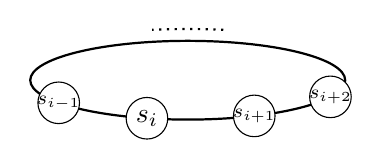
\begin{tikzpicture}[yscale=0.25, spins/.style={draw, fill=white, shape=circle}] %, baseline=(x.base)]    \node (x) at (0,0) {\vphantom{x}};

        \draw[thick] (0,0) circle[radius=2cm];
        \draw[thick, dotted] (80:2.6) arc[start angle=80, end angle=100, radius=2.6];

        %\draw[fill=white] (215:2) node {$s_{i-1}$} circle[radius=0.3cm];
        %\draw[fill=white] (255:2) node {$s_i$} circle[radius=0.3cm];
        %\draw[fill=white] (295:2) node {$s_{i+1}$} circle[radius=0.3cm];
        %\draw[fill=white] (335:2) node {$s_{i+2}$} circle[radius=0.3cm];


        \node[spins] at (215:2) {\vphantom{X}};\node at (215:2) {\scriptsize $s_{i-1}$};
        \node[spins] at (255:2) {\vphantom{X}};\node at (255:2) {$s_i$};
        \node[spins] at (295:2) {\vphantom{X}};\node at (295:2) {\scriptsize $s_{i+1}$};
        \node[spins] at (335:2) {\vphantom{X}};\node at (335:2) {\scriptsize $s_{i+2}$};

    \end{tikzpicture}
  }
  \qquad\qquad
  \subfloat[\label{fig:Ising_q}]{
      \begin{tikzpicture}[yscale=0.25, spins/.style={draw, fill=white, shape=circle}] %, baseline=(x.base)]    \node (x) at (0,0) {\vphantom{x}};

        \draw[thick] (0,0) circle[radius=2cm];
        \draw[thick, dotted] (80:2.6) arc[start angle=80, end angle=100, radius=2.6];

        \node (si-1) at (215:2) {\large$\bullet$};\node (i-1) at ($(si-1)+(0.1,1.4)$) {$\mathbb{C}^2$};
        \node (si) at (255:2) {\large$\bullet$};\node (i) at ($(si)+(0.1,1.5)$) {$\mathbb{C}^2$};
        \node (si+1) at (295:2) {\large$\bullet$};\node (i+1) at ($(si+1)+(0,1.5)$) {$\mathbb{C}^2$};
        \node (si+2) at (335:2) {\large$\bullet$};\node (i+2) at ($(si+2)+(-0.2,1.2)$) {$\mathbb{C}^2$};

%        \draw[thick, arrows=-to] (i-1) to node[below left] {$T$} (i);
%        \draw[thick, arrows=-to] (i) to node[below] {$T$} (i+1);
%        \draw[thick, arrows=-to] (i+1) to node[below right] {$T$} (i+2);

    \end{tikzpicture}
  }
  \caption{(a) Classical Ising spin chain. Spin variables $s_i$ take values in $\{ \pm1 \}$.
  They are just $c$ numbers. (b) Quantum spins are vectors in $\C^2$ associated at each site.
  The discrete time evolution of quantum spins is given by the transfer matrix.}
  \label{fig:1d_Ising}
\end{figure}


Now introduce the \emph{transfer matrix},
\begin{equation}
  T  :=  \left(e^{Kss'}\right)_{s,s'=\pm1}
    =
    \left(\begin{array}{ll}
  e^{K}  &  e^{-K}  \\
  e^{-K}  &  e^{K}
\end{array}\right),
\end{equation}
where the indices of row and column are labeled by $+1$ and $-1$,
respectively. Using this matrix $T$, the partition function is rewritten
as
\begin{equation}
  Z\left(\beta\right)
    =\sum_{s_{1},\ldots,s_{n}=\pm1}  T_{s_{1}s_{n}}  \cdots  T_{s_{3}s_{2}}T_{s_{2}s_{1}}.
\end{equation}
By definition of matrix multiplication, the partition function is
eventually given by a trace:
\begin{align}
  Z(\beta)
  & =  \sum_{s_{1}=\pm1}\left(T^{n}\right)_{s_{1}s_{1}}  \nonumber \\
  & =  \mathrm{Tr}_{\mathbb{C}^{2}}\left(T^{n}\right).
\end{align}
This expression tells us that we have the quantum Hilbert space $\mathbb{C}^{2}$
at the boundary of each 1d segment, and the transfer matrix $T$ sends
a state to the adjacent site, which is the discrete ``time evolution''
of this system; $\log T\propto$ Hamiltonian as we saw in 1d QFT in
section \ref{sec:what_is_qft}. This corresponds to the analogue of Hamiltonian/operator
formalism in field theory. In operator formalism, spins
are replaced by the Pauli matrices, and original classical up spin
and down spin are replaced by the eigenvalues and eigenvectors of
the Pauli matrix $\sigma^{z}$. Further, the non-commutativity is
now manifest in a way that the spins and their time evolution is given
by matrices, this is the consequence of quantization.

In the expression above of the partition function, let us consider
the thermodynamic limit $n\to\infty$. The eigenvalues of
$T$ are easily obtained and let them be $\lambda_{0}>\lambda_{1}$,
then we have the free energy
\begin{align}
-\beta f(\beta)
  & =  \lim_{n\to\infty}\frac{1}{n}\log Z(\beta)\nonumber \\
  & =  \lim_{n\to\infty}\frac{1}{n}\log\lambda_{0}\left(1+\left(\frac{\lambda_{1}}{\lambda_{0}}\right)^{n}\right)\nonumber \\
  & =  \log\lambda_{0}.
\end{align}
We conclude that the free energy in the thermodynamic limit is just
given by the largest eigenvalue of the transfer matrix. Finally, integrability
of lattice model is rephrased as
\begin{align*}
  &  \textrm{One can exatly find the eigenvalues of transfer matrix.} \\
  &  \Rightarrow  ~  \textrm{Can exactly compute the free enrgy.} \\
  &  \Rightarrow  ~  \textrm{The system is exactly solvable.}
\end{align*}

The transfer matrices of 1d and 2d Ising model are diagonalizable
and one can exactly find their eigenvectors and eigenvalues using,
for example, algebraic Bethe ansatz. In this sense, 1d and 2d Ising
model are said to be integrable, or exactly solvable. Then, a natural
question arises; when can we diagonalize the transfer matrix of a
lattice model? This actually leads to the most fundamental answer
to the question of ``what is integrable model.'' A canonical answer
is \emph{Yang-Baxter equation}. When the Boltzmann weight with spectral
parameters, which take values in a Riemann surface, satisfies the
Yang-Baxter equation, the lattice model is integrable. We are going to give
an explanation of this definition of integrability in next subsection
in some detail, with its origin from TQFT with extra dimensions.


%FIGURE
%\begin{figure}[tbp]
%\centering
%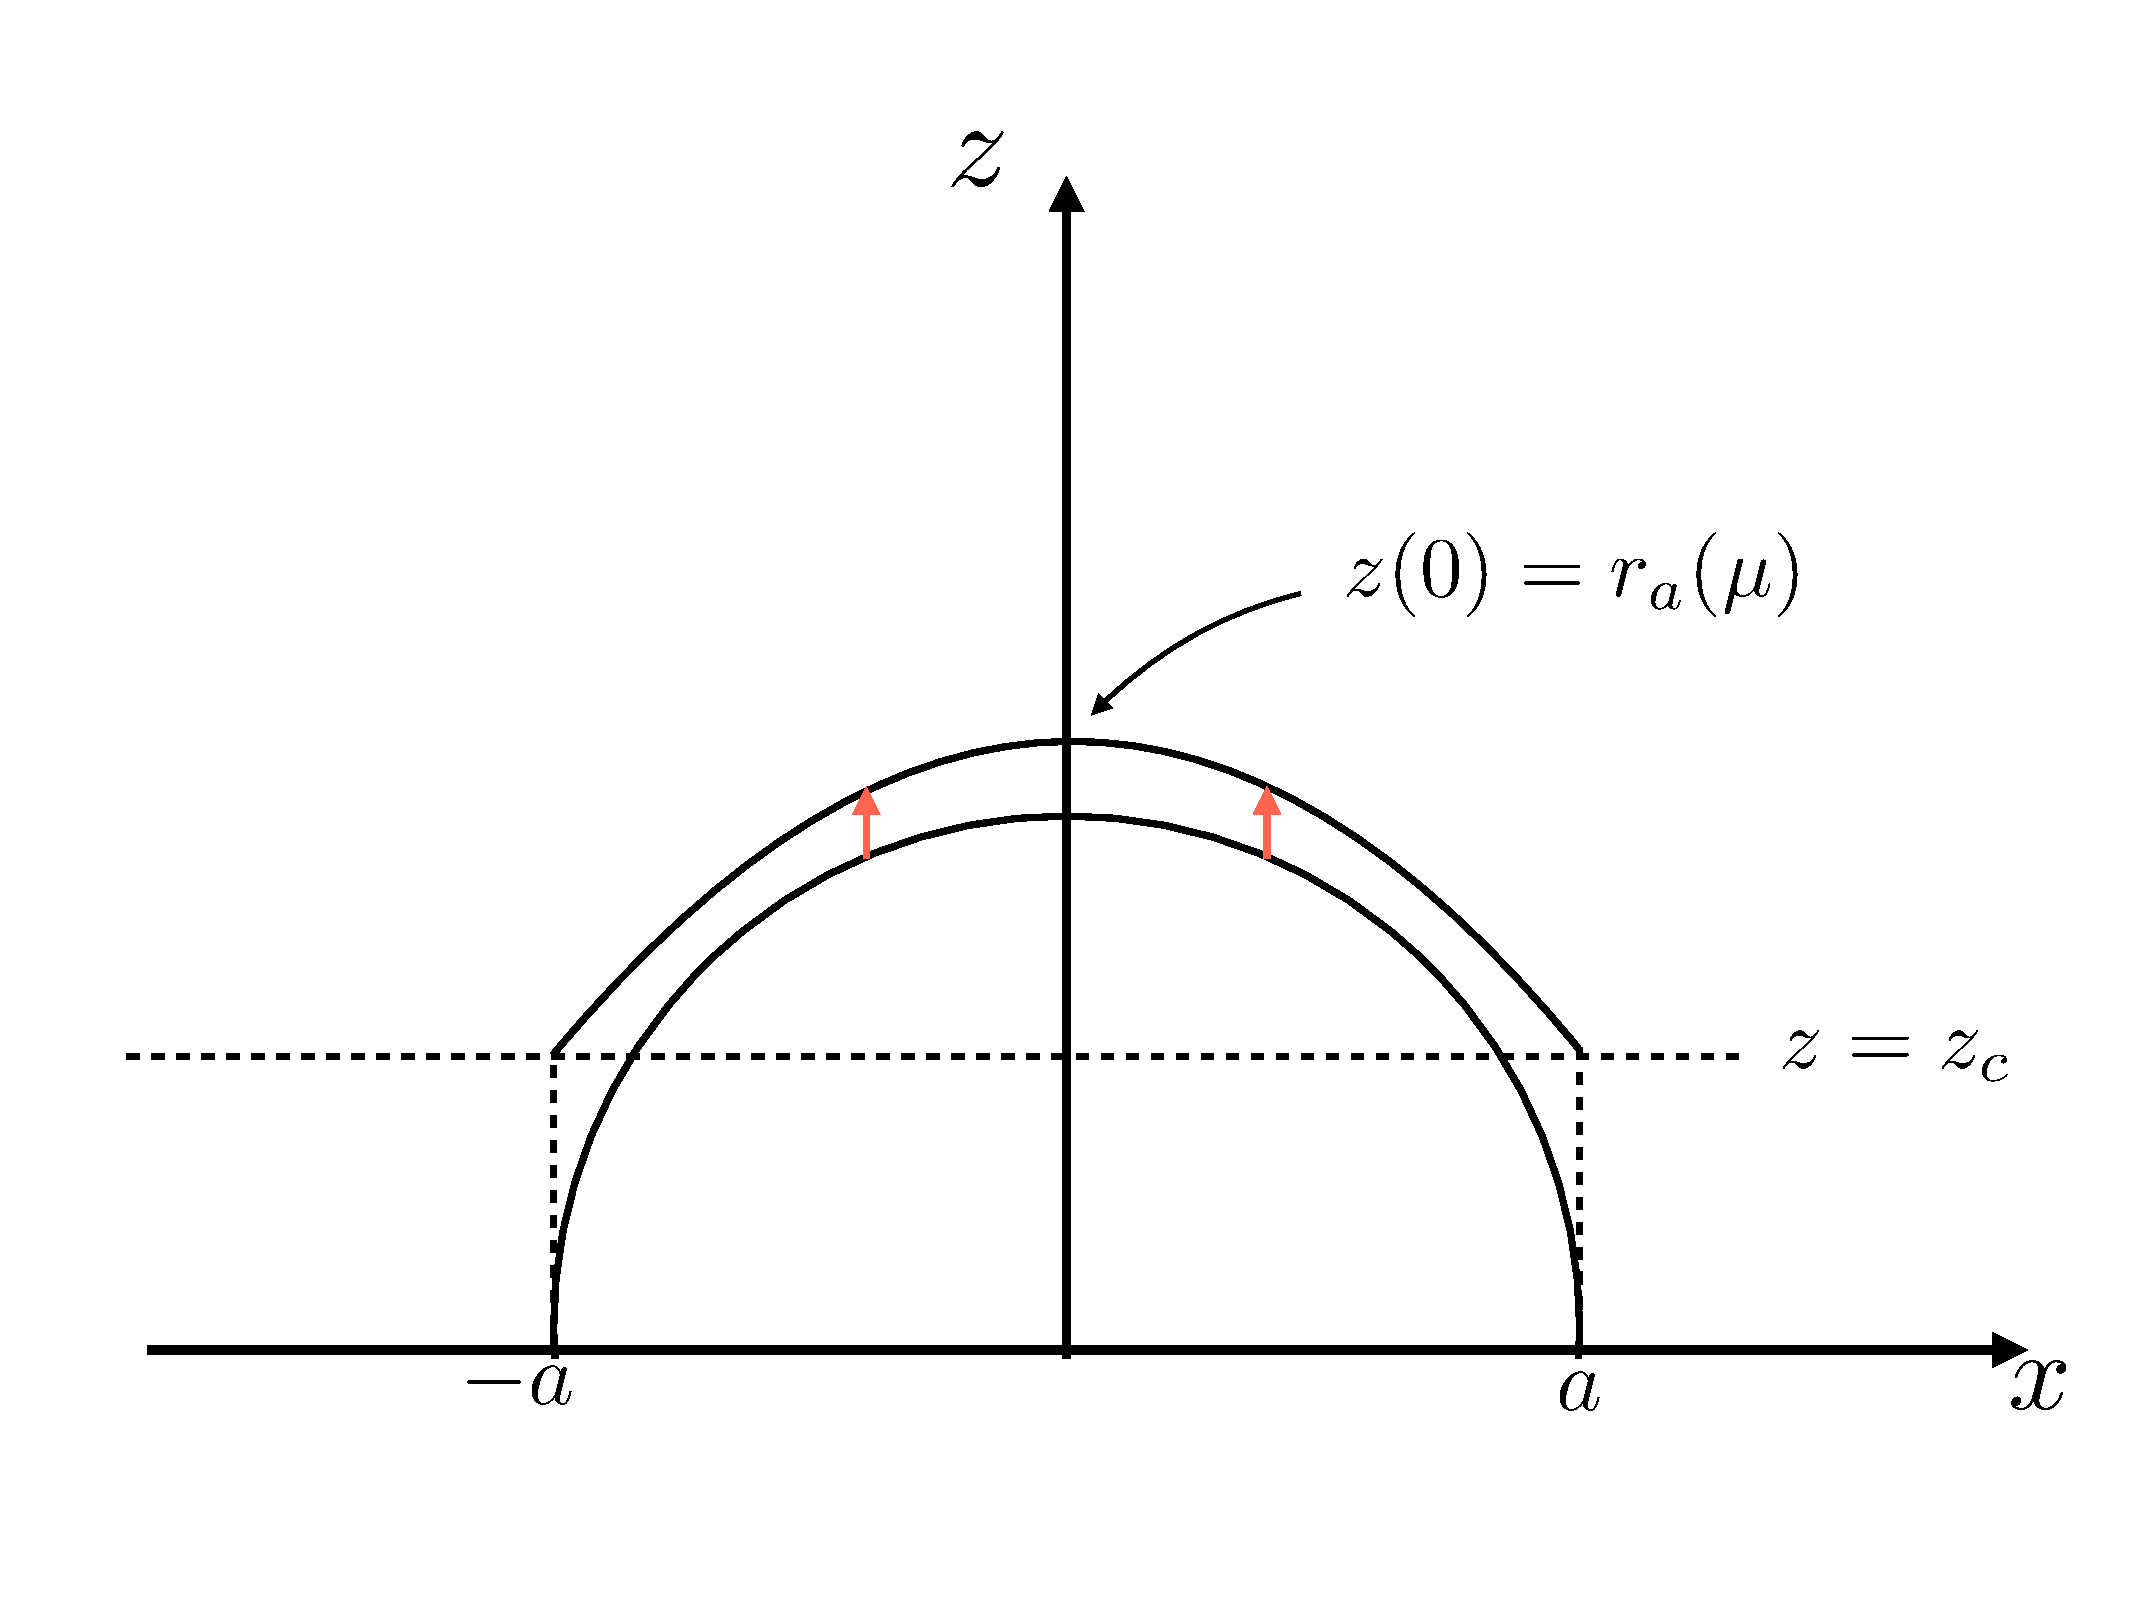
\includegraphics[width=6cm, trim=5cm 4cm 5cm 2cm]{fig/EE1.pdf}
%\caption{A deformed geodesic in the $T\bar{T}$ deformed geometry. }
%\label{fig:deformed}
%\end{figure}





\subsection{Integrability from TQFT in extra dimensions}
\label{sec:integrability_from_TQFT}

So far, we have seen that a QFT is ideally given by some functor $Z$, and
lattice model is also given by $Z$ as a discrete version of QFT.
Now, we would like to relate these two. The key concept is that
``line operators in 2d TQFT form a lattice model.''
In particular, if the 2d TQFT has extra dimensions, a corresponding
lattice model naturally turns out to be integrable.


The purpose of this section is to provide a general discussion to relate four-dimensional
supersymmetric gauge theories and integrable lattice models.
We first give a step-by-step
explanation from two-dimensional TQFT to integrable lattice model,
and then put the argument in the setup of brane tilings. Branes in
string theory are powerful enough to yield the systematic method to
relate a class of supersymmetric gauge theories with integrable lattice
models, as we will see. To begin with, we present a general prescription
of brane constructions at a formal level. Concrete setups and more
details will be given in later sections.
The discussion in this subsection is mainly based on \cite{Yagi:2016oum}.





\subsubsection{Lattice models from TQFTs with line operators}

Suppose that we have a two-dimensional TQFT $\mathsf{T}$ on a two-torus
$T^{2}$ equipped with line operators $\mathcal{L}_{i}$, $i=1,\ldots,l$.
Wrap them around one-cycles $C_{i}$ on the torus in such a way that
they form an $m\times n$ lattice; see figure \ref{fig:line_on_torus}. We wish to consider the correlation
function of this configuration of line operators. To compute it, our
strategy is to break up the torus into pieces and perform in turn
the path integral piecewise. Then the original correlation function
is reconstructed by combining these pieces.%
%
\footnote{The original Atiyah's TQFT is actually called ``closed TQFT.''
In the following, we will compute the correlation function by embedding
the closed TQFT with line operators into an open/closed TQFT with
line operators, or so-called defect TQFT; see e.g.~\cite{Moore:2006dw,Carqueville:2016nqk}. }
%

Let us consider the following piece of surface which contains an intersection
of two line operators $\mathcal{L}_{i}$ and $\mathcal{L}_{j}$:
\begin{equation}
  \label{eq:piece_of_lines}
    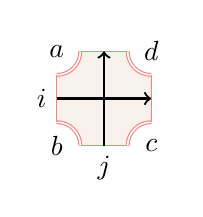
\begin{tikzpicture}[scale=0.6, baseline=(x.base)]
        \node (x) at (0,0) {\vphantom{x}};

        \draw[color=red!50, fill=brown!10] (-1,-1) rectangle (1,1);

        \fill[color=white] (-1,1) circle (0.5);  \node (a) at (-1,1) {$a$};
        \draw[draw=red!50, double]  (-1,0.5) arc (-90:0:0.5);
        \fill[color=white] (-1,-1) circle (0.5);  \node (b) at (-1,-1) {$b$};
        \draw[draw=red!50, double]  (-1,-0.5) arc (90:0:0.5);
        \fill[color=white] (1,-1) circle (0.5);  \node (c) at (1,-1) {$c$};
        \draw[draw=red!50, double]  (1,-0.5) arc (90:180:0.5);
        \fill[color=white] (1,1) circle (0.5);  \node (d) at (1,1) {$d$};
        \draw[draw=red!50, double]  (1,0.5) arc (-90:-180:0.5);

        \draw[thick, ->] (-1,0) node[left] {$i$} -- (1,0);
        \draw[thick, ->] (0,-1) node[below] {$j$} -- (0,1);

    \end{tikzpicture}
  \quad .
\end{equation}
If one thinks of the above picture as the world-sheet of two scattering
open strings, one can regard the above picture as follows: The endpoints
of the open strings sweep out the double-lined arcs, on which D-branes
are there and the boundary conditions (Chan-Paton factors) are specified
by labels $a,\,b,\,c,\,d$. The line operators are the world-lines
of particles associated with the open strings.


%FIGURE
\begin{figure}
  \centering
  \subfloat[\label{fig:line_on_torus}]{
    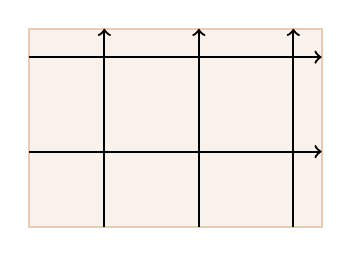
\begin{tikzpicture}[scale=1.2, bdy/.style={draw, color=red, double, fill=white, shape=circle}] %, baseline=(x.base)]  \node (x) at (0,0) {\vphantom{x}};
        \def\width{3.1cm}
        \def\height{2.1cm}

        \filldraw[color=brown!40, semithick, fill=brown!10] (0,0) rectangle (\width,\height);
        \draw[thick, ->, black] (0.8,0) -- ++(0,\height);\draw[thick, ->, black] (1.8,0) -- ++(0,\height);\draw[thick, ->, black] (2.8,0) -- ++(0,\height);
        \draw[thick, ->, black] (0,0.8) -- ++(\width,0);\draw[thick, ->, black] (0,1.8) -- ++(\width,0);

    \end{tikzpicture}
  }
  \qquad
  \subfloat[\label{fig:line_boundary}]{
    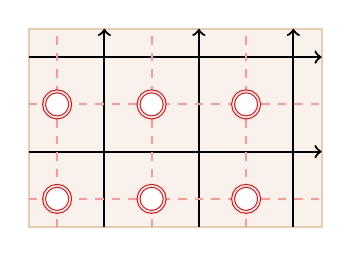
\begin{tikzpicture}[scale=1.2, bdy/.style={draw, color=red, double, fill=white, shape=circle}] %, baseline=(x.base)]
%        \node (x) at (0,0) {\vphantom{x}};
        \def\width{3.1cm}
        \def\height{2.1cm}

        \filldraw[color=brown!40, semithick, fill=brown!10] (0,0) rectangle (\width,\height);
        \draw[thick, ->, black] (0.8,0) -- ++(0,\height);\draw[thick, ->, black] (1.8,0) -- ++(0,\height);\draw[thick, ->, black] (2.8,0) -- ++(0,\height);
        \draw[thick, ->, black] (0,0.8) -- ++(\width,0);\draw[thick, ->, black] (0,1.8) -- ++(\width,0);

        \draw[thick, color=red!40, dashed] (0.3,0) -- ++(0,\height);\draw[thick, color=red!40, dashed] (1.3,0) -- ++(0,\height);\draw[thick, color=red!40, dashed] (2.3,0) -- ++(0,\height);
        \draw[thick, color=red!40, dashed] (0,0.3) -- ++(\width,0);\draw[thick, color=red!40, dashed] (0,1.3) -- ++(\width,0);

        \node[bdy] (b1) at (0.3,0.3) {};
        \node[bdy] (b2) at (1.3,0.3) {};
        \node[bdy] (b3) at (2.3,0.3) {};
        \begin{scope}[yshift=1cm]
        \node[bdy] at (0.3,0.3) {};
        \node[bdy] at (1.3,0.3) {};
        \node[bdy] at (2.3,0.3) {};
        \end{scope}

    \end{tikzpicture}
  }
  \qquad
  \subfloat[\label{fig:spin_boundary}]{
    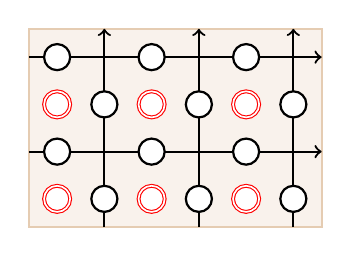
\begin{tikzpicture}[scale=1.2, bdy/.style={draw, color=red, double, fill=white, shape=circle},spin/.style={draw, thick, fill=white, shape=circle}] %, baseline=(x.base)]
%        \node (x) at (0,0) {\vphantom{x}};
        \def\width{3.1cm}
        \def\height{2.1cm}

        \filldraw[color=brown!40, semithick, fill=brown!10] (0,0) rectangle (\width,\height);
        \draw[thick, ->, black] (0.8,0) -- ++(0,\height);\draw[thick, ->, black] (1.8,0) -- ++(0,\height);\draw[thick, ->, black] (2.8,0) -- ++(0,\height);
        \draw[thick, ->, black] (0,0.8) -- ++(\width,0);\draw[thick, ->, black] (0,1.8) -- ++(\width,0);

        \node[bdy] (b1) at (0.3,0.3) {};\node[bdy] (b2) at (1.3,0.3) {};\node[bdy] (b3) at (2.3,0.3) {};
        \begin{scope}[yshift=1cm]
        \node[bdy] at (0.3,0.3) {};\node[bdy] at (1.3,0.3) {};\node[bdy] at (2.3,0.3) {};
        \end{scope}

        \begin{scope}[xshift=0.5cm]
        \node[spin] at (0.3,0.3) {};\node[spin] at (1.3,0.3) {};\node[spin] at (2.3,0.3) {};
        \end{scope}
        \begin{scope}[yshift=0.5cm]
        \node[spin] at (0.3,0.3) {};\node[spin] at (1.3,0.3) {};\node[spin] at (2.3,0.3) {};
        \end{scope}
        \begin{scope}[yshift=1cm]
                \begin{scope}[xshift=0.5cm]
                \node[spin] at (0.3,0.3) {};\node[spin] at (1.3,0.3) {};\node[spin] at (2.3,0.3) {};
                \end{scope}
                \begin{scope}[yshift=0.5cm]
                \node[spin] at (0.3,0.3) {};\node[spin] at (1.3,0.3) {};\node[spin] at (2.3,0.3) {};
                \end{scope}
        \end{scope}
    \end{tikzpicture}
  }
  \caption{Construction of a lattice model from line operators.
    (a) A lattice of line operators on a torus.
    (b) The torus with holes obtained by gluing the pieces.
    (c) The corresponding spin model. }
  \label{fig:TQFT_and_Spin}
\end{figure}


The path integral for the piece \eqref{eq:piece_of_lines} produces a linear map
(recall an important property of quantum mechanics \eqref{eq:qm_linearmap} and
an assignment of TQFT)
\begin{equation}
    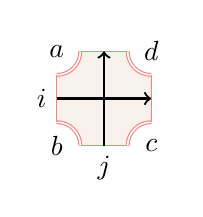
\begin{tikzpicture}[scale=0.6, baseline=(x.base)]
        \node (x) at (0,0) {\vphantom{x}};

        \draw[color=red!50, fill=brown!10] (-1,-1) rectangle (1,1);

        \fill[color=white] (-1,1) circle (0.5);  \node (a) at (-1,1) {$a$};
        \draw[draw=red!50, double]  (-1,0.5) arc (-90:0:0.5);
        \fill[color=white] (-1,-1) circle (0.5);  \node (b) at (-1,-1) {$b$};
        \draw[draw=red!50, double]  (-1,-0.5) arc (90:0:0.5);
        \fill[color=white] (1,-1) circle (0.5);  \node (c) at (1,-1) {$c$};
        \draw[draw=red!50, double]  (1,-0.5) arc (90:180:0.5);
        \fill[color=white] (1,1) circle (0.5);  \node (d) at (1,1) {$d$};
        \draw[draw=red!50, double]  (1,0.5) arc (-90:-180:0.5);

        \draw[thick, ->] (-1,0) node[left] {$i$} -- (1,0);
        \draw[thick, ->] (0,-1) node[below] {$j$} -- (0,1);

    \end{tikzpicture}
  \quad \rightsquigarrow \quad
R_{ij}\left(%
  \begin{array}{cc}
        a & d\\
        b & c
  \end{array}%
\right)
  :  V_{ab,i}\otimes V_{bc,j}  \longrightarrow  V_{ad,j}\otimes V_{dc,i} \, ,
\end{equation}
where $V_{ab,i}$ is the space of states of the open string propagating
along $\mathcal{L}_{i}$ with the boundary conditions on the left
and the right ends specified by $a,\,b$, respectively. We call this
map the R-matrix (or R-operator) associated with this decorated surface.
To reconstruct the original configuration of line operators, we glue these
pieces together. Gluing them amounts to the composition of R-matrices.
For example, gluing two pieces horizontally gives
\begin{equation}
    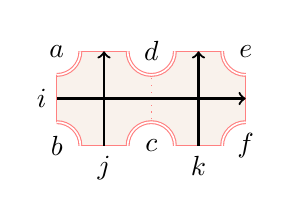
\begin{tikzpicture}[scale=0.6, baseline=(x.base)]  \node (x) at (0,0) {\vphantom{x}};

        \draw[color=red!50, fill=brown!10] (-1,-1) rectangle (3,1);
        \draw[color=red!50, dotted] (1,-1) -- (1,1);

        \fill[color=white] (-1,1) circle (0.5);  \node (a) at (-1,1) {$a$};
        \draw[draw=red!50, double]  (-1,0.5) arc (-90:0:0.5);
        \fill[color=white] (-1,-1) circle (0.5);  \node (b) at (-1,-1) {$b$};
        \draw[draw=red!50, double]  (-1,-0.5) arc (90:0:0.5);
        \fill[color=white] (1,-1) circle (0.5);  \node (c) at (1,-1) {$c$};
        \draw[draw=red!50, double]  (1.5,-1) arc (0:180:0.5);
        \fill[color=white] (1,1) circle (0.5);  \node (d) at (1,1) {$d$};
        \draw[draw=red!50, double]  (1.5,1) arc (0:-180:0.5);
        \fill[color=white] (3,-1) circle (0.5);  \node (f) at (3,-1) {$f$};
        \draw[draw=red!50, double]  (3,-0.5) arc (90:180:0.5);
        \fill[color=white] (3,1) circle (0.5);  \node (e) at (3,1) {$e$};
        \draw[draw=red!50, double]  (3,0.5) arc (-90:-180:0.5);

        \draw[thick, ->] (-1,0) node[left] {$i$} -- (3,0);
        \draw[thick, ->] (0,-1) node[below] {$j$} -- (0,1);
        \draw[thick, ->] (2,-1) node[below] {$k$} -- (2,1);

    \end{tikzpicture}
%  \ =
\quad \rightsquigarrow \quad
R_{ik}\left(%
  \begin{array}{cc}
        d & e\\
        c & f
  \end{array}%
\right)
  \circ_{V_{dc,i}}
R_{ij}\left(%
  \begin{array}{cc}
        a & d\\
        b & c
  \end{array}%
\right).
\end{equation}

The original configuration is thus obtained by gluing all the pieces.
It, however, still has holes assigned boundary conditions as in figure \ref{fig:line_boundary},
which we must fill by summing over the boundary conditions. To do
this, let us recall that the path integral on a finite-length cylinder
with boundary condition $a$ imposed on one end defines a closed string
state $\left|a\right\rangle $ as known as a boundary state. Similarly,
the path integral on a disk with no insertion of operators defines
a state $\left|1\right\rangle $ on the boundary.
%, see figures.
Assume
that we have chosen the set of boundary conditions $B$ to be sufficiently
large so that the state $\left|1\right\rangle $ can be written as
a superposition of boundary states:
\begin{equation}
  \left|1\right\rangle  =  \sum_{a\in B}c_{a}\left|a\right\rangle .
\end{equation}
Then, the sum over the boundary conditions gives the state $\left|1\right\rangle $
on the boundary of each hole, which is replaced with a disk:
\begin{equation}
  \sum_{a\in B}  c_a  \left(  ~  a  ~
    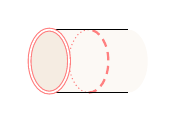
\begin{tikzpicture}[xscale=0.25, yscale=0.4, baseline=(x.base)]
        \node (x) at (0,0) {\vphantom{x}};
        \def\cylinderlength{4cm}

        \fill[color=brown!5] (0,-1) arc (-90:90:1) -- ++(\cylinderlength,0) arc (90:-90:1) -- ++(-\cylinderlength,0) -- cycle;

        \draw[color=red!50, densely dashed, thick] (\cylinderlength/2,-1) arc (-90:90:1);
        \draw[color=red!50, densely dotted] (\cylinderlength/2,1) arc (90:270:1);

        \draw (0,1) -- (\cylinderlength,1);
        \draw (0,-1) -- (\cylinderlength,-1);

        \filldraw[color=red!50, double, fill=brown!15] (0,0) circle[radius=1];

    \end{tikzpicture}
  \right)
  =
  \sum_{a\in B}  c_a  \left(  ~  \left|a\right\rangle  ~
    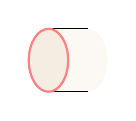
\begin{tikzpicture}[xscale=0.25, yscale=0.4, baseline=(x.base)]
        \node (x) at (0,0) {\vphantom{x}};
        \def\cylinderlength{2cm}

        \fill[color=brown!5] (0,-1) arc (-90:90:1) -- ++(\cylinderlength,0) arc (90:-90:1) -- ++(-\cylinderlength,0) -- cycle;

        \draw (0,1) -- (\cylinderlength,1);
        \draw (0,-1) -- (\cylinderlength,-1);

%        \draw[color=red!50, densely dashed, thick] (\cylinderlength/2,-1) arc (-90:90:1);
%        \draw[color=red!50, densely dotted] (\cylinderlength/2,1) arc (90:270:1);

        \filldraw[color=red!50, thick, fill=brown!15] (0,0) circle[radius=1];

    \end{tikzpicture}
  \right)
    =  ~
    \left|1\right\rangle  ~
      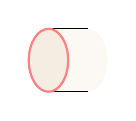
\begin{tikzpicture}[xscale=0.25, yscale=0.4, baseline=(x.base)]
        \node (x) at (0,0) {\vphantom{x}};
        \def\cylinderlength{2cm}

        \fill[color=brown!5] (0,-1) arc (-90:90:1) -- ++(\cylinderlength,0) arc (90:-90:1) -- ++(-\cylinderlength,0) -- cycle;

        \draw (0,1) -- (\cylinderlength,1);
        \draw (0,-1) -- (\cylinderlength,-1);
        \filldraw[color=red!50, thick, fill=brown!15] (0,0) circle[radius=1];

    \end{tikzpicture}
  \ = \
    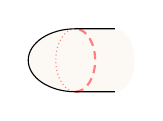
\begin{tikzpicture}[xscale=0.25, yscale=0.4, baseline=(x.base)]
        \node (x) at (0,0) {\vphantom{x}};
        \def\cylinderlength{2cm}

        \fill[color=brown!5] (0,-1)  arc[start angle=270,end angle=90,x radius=2.4,y radius=1] -- ++(\cylinderlength,0) arc (90:-90:1) -- ++(-\cylinderlength,0) -- cycle;

        \draw[color=red!50, densely dashed, thick] (0,-1) arc (-90:90:1);
        \draw[color=red!50, densely dotted] (0,1) arc (90:270:1);

        \draw (\cylinderlength,-1) -- (0,-1) arc[start angle=270,end angle=90,x radius=2.4,y radius=1]   -- (\cylinderlength,1);

    \end{tikzpicture}
  \quad  .
\end{equation}
Thus the holes are filled and the original configuration on the torus
is reconstructed.

Now that we have understood how to reconstruct the correlation function
of line operators in the field theoretic point of view, let us reinterpret
this procedure as an operation in statistical lattice model. Rephrasing
the procedures so far, it is clear that the above configuration defines
a partition function of a statistical spin model. The model has spins
located at two kinds of sites, \tikz{\draw[thick, fill=white] (0,0) circle[radius=0.15cm]}
and \tikz{\draw[semithick, double, fill=white] (0,0) circle[radius=0.14cm]}. They
correspond to the open string states and the boundary states, see figure \ref{fig:spin_boundary}.
A spin
at \tikz{\draw[thick, fill=white] (0,0) circle[radius=0.15cm]} takes values in the chosen basis for the relevant open
string states $V_{ab,i}$, while that at \tikz{\draw[semithick, double, fill=white] (0,0) circle[radius=0.14cm]} is valued
in $B$. The Boltzmann weights for each spin configuration are given
by the matrix elements of R-matrix and the coefficients of boundary
states $c_{a}$. Thus, we conclude that the correlation function of
line operators $\{ \mathcal{L}_{i}\} $ on the torus coincides
with the partition function of a statistical spin model defined on
the periodic lattice formed by the line operators:
\begin{equation}
  \left\langle  \prod_{i=1}^{l}\mathcal{L}_{i}[C_i]  \right\rangle_{\mathsf{T},T^{2}}
    =
      Z_{\mathsf{L}(\mathsf{T})} \big( \{ \mathcal{L}_{i}[C_i]\} \big).
\end{equation}
$\mathsf{L}(\mathsf{T})$ denotes the lattice model arising
from the TQFT $\mathsf{T}$ with the line operators and $\{ \mathcal{L}_{i}[C_i]\} $
is the lattice formed by line operators $\mathcal{L}_{i}$ wrapping
around $C_{i}$.
In other words, the partition function of lattice model \eqref{eq:lattice_Z}
is in this case defined by the lattice $\{ \mathcal{L}_{i}[C_i]\} $, and specified by the left-hand side.
By this construction, we can view typical examples
of lattice models.

\subsubsection*{IRF model}

If $\dim V_{ab,i}=1$ for any $a,\,b,\,i$, in this case we can ignore
the spins at \tikz{\draw[thick, fill=white] (0,0) circle[radius=0.15cm]}. We just sum over the boundary conditions
and such a spin system $\mathsf{L}(\mathsf{T})$ is called
\emph{interaction-round-a-face model}, or \emph{IRF model} for short.
The spins are placed on the faces of the lattice, and interaction
takes place among four spins surrounding a vertex. The 2d Ising model
actually can be formulated as an IRF model by taking vertex-face transformation.


\subsubsection*{Vertex model}

If $B$ consists of a single boundary condition, say $a$, we can
simply write the open string state space by $V_{i}:=V_{aa,i}$, and
the R-matrix is represented only by a crossing of two lines:
\begin{equation}
  R_{ij}
  =
    \begin{tikzpicture}[scale=0.6, baseline=(x.base)]
        \node (x) at (0,0) {\vphantom{x}};

        \draw[thick, ->] (0,0) node[left] {$i$} -- (2,0);
        \draw[thick, ->] (1,-1) node[below] {$j$} -- (1,1);

    \end{tikzpicture}
  \quad ,
\end{equation}
\begin{equation}
  R_{ij}  :  V_{i}\otimes V_{j}  \longrightarrow  V_{j}\otimes V_{i}
  ~ .
\end{equation}
The space of states $V_{i}$ can also be thought of as the Hilbert
space of a particle propagating on the line operator $\mathcal{L}_{i}$.
In this case we can ignore the spins at \tikz{\draw[semithick, double, fill=white] (0,0) circle[radius=0.14cm]} since there
is no summation over boundary conditions. This means that the lattice
model $\mathsf{L}\left(\mathsf{T}\right)$ is called a \emph{vertex
model}: Spins are living on the edges of the lattice and interact
with each other at the vertices.

We can always recast our lattice model into a vertex model by setting
$V_{i}:=\bigoplus_{a,b\in B}V_{ab,i}$, at least formally, and declaring
that all newly introduced R-matrix elements, which correspond to scattering
processes with inconsistent Chan-Paton factors, vanish. We can also
absorb the coefficients $c_{a}$ into the R-matrix elements by appropriate
rescaling. In what follows we implicitly perform this reformulation,
and restrict ourselves to vertex model.

A remarkable aspect of this construction of lattice models is that
it allows us to understand integrability from a higher-dimensional
point of view. This is crucial observation by Costelllo \cite{Costello:2013sla}.
In our lattice model, consider a horizontal line operator $\mathcal{L}_{i}$
intersecting vertical line operators $\mathcal{L}_{j}$, $j=1,\ldots,n$.
Concatenating the R-matrices in this row, we get the row-to-row transfer
matrix:
\begin{equation}
  T_{i}
  =
    \begin{tikzpicture}[scale=0.8, baseline=(x.base)]
        \node (x) at (0,0) {\vphantom{x}};

        \draw[thick] (0,0) arc (270:90:0.1);
        \draw[thick, ->-=0.24] (0,0) node[left] {$i~$} -- (3,0);
        \draw[thick] (3,0) arc (-90:90:0.1);

        \draw[preaction={draw=white, ultra thick}, thick, loosely dotted] (1.2,0) -- (2.4,0);

        \draw[thick, ->] (0.3,-0.4) node[below] {$1$} -- (0.3, 0.6);
        \draw[thick, ->] (0.9,-0.4) node[below] {$2$} -- (0.9, 0.6);
        \draw[thick, ->] (2.7,-0.4) node[below] {$n$} -- (2.7, 0.6);

    \end{tikzpicture}
  \ =
  \mathrm{Tr}_{V_{i}}\left(R_{i,n}\circ_{V_{i}}\cdots\circ_{V_{i}}R_{i,1}\right).
\end{equation}
The hooks on the horizontal line are to remind us that the periodic
boundary condition is imposed. This gives an endomorphism of $\bigotimes_{j=1}^{n}V_{j}$
which maps a state just below $\mathcal{L}_{j}$ to another state
above it, namely the transfer matrix defines the discrete time evolution of
this spin system and $\mathcal{H}:=\bigotimes_{j=1}^{n}V_{j}$ is the total quantum Hilbert
space. In terms of transfer matrices, the partition function is written
as a trace,
\begin{equation}
  Z_{\mathsf{L}(\mathsf{T})} \big( \{ \mathcal{L}_{i}[C_i]\}  \big)
  =\mathrm{Tr}_{\mathcal{H}}\left(T_{n+m}\cdots T_{n+1}\right).
\end{equation}
An important point is that the underlying field theory is a TQFT,
and hence a state evolves trivially on a cylinder unless it hits something,
line operators in the present case.

Now suppose that each line operator depends on a continuous parameter
which is an element of some smooth manifold $S$. This parameter is
called \emph{spectral parameter} of the lattice model. Let $u_{i}$ be the
spectral parameter of $\mathcal{L}_{i}$, then the R-matrix
and the transfer matrix are rewritten by
\begin{align}
  R_{ij}  &  \longrightarrow R_{ij}(u_{i},u_{j}),  \\
  T_{i}   &  \longrightarrow T_{i}(u_{i};u_{1},\ldots,u_{n}).
\end{align}
To avoid clutter, we fix $u_{1},\ldots,u_{n}$ and suppress them
below. A vertex model is said to be integrable if the transfer matrices
$T_{i}(u_{i})$ are meromorphic functions of $u_{i}$ and
commute with each other:
\begin{equation}
    \begin{tikzpicture}[xscale=0.8, yscale=0.6, baseline=(x.base)]
        \node (x) at (0,0.5) {\vphantom{x}};

        \draw[thick, ->] (0.3,-0.4) -- (0.3, 1.6);
        \draw[thick, ->] (0.9,-0.4) -- (0.9, 1.6);
        \draw[thick, ->] (2.7,-0.4) -- (2.7, 1.6);
        %arrows do not work somehow by preaction below

        \draw[thick] (0,0) arc (270:90:0.1);
        \draw[thick, ->-=0.24] (0,0) node[left] {$i~$} -- (3,0);
        \draw[thick] (3,0) arc (-90:90:0.1);
        \draw[preaction={draw=white, ultra thick}, thick, loosely dotted] (1.2,0) -- (2.4,0);

        \draw[thick, yshift=1cm] (0,0) arc (270:90:0.1);
        \draw[thick, ->-=0.24, yshift=1cm] (0,0) node[left] {$j~$} -- (3,0);
        \draw[thick, yshift=1cm] (3,0) arc (-90:90:0.1);
        \draw[preaction={draw=white, ultra thick}, thick, loosely dotted, yshift=1cm] (1.2,0) -- (2.4,0);

    \end{tikzpicture}
  \ =
    \begin{tikzpicture}[xscale=0.8, yscale=0.6, baseline=(x.base)]
        \node (x) at (0,0.5) {\vphantom{x}};

        \draw[thick, ->] (0.3,-0.4) -- (0.3, 1.6);
        \draw[thick, ->] (0.9,-0.4) -- (0.9, 1.6);
        \draw[thick, ->] (2.7,-0.4) -- (2.7, 1.6);
        %arrows do not work somehow by preaction below

        \draw[thick] (0,0) arc (270:90:0.1);
        \draw[thick, ->-=0.24] (0,0) node[left] {$j~$} -- (3,0);
        \draw[thick] (3,0) arc (-90:90:0.1);
        \draw[preaction={draw=white, ultra thick}, thick, loosely dotted] (1.2,0) -- (2.4,0);

        \draw[thick, yshift=1cm] (0,0) arc (270:90:0.1);
        \draw[thick, ->-=0.24, yshift=1cm] (0,0) node[left] {$i~$} -- (3,0);
        \draw[thick, yshift=1cm] (3,0) arc (-90:90:0.1);
        \draw[preaction={draw=white, ultra thick}, thick, loosely dotted, yshift=1cm] (1.2,0) -- (2.4,0);

    \end{tikzpicture}
%\end{equation}
%\begin{equation}
~ \Longleftrightarrow ~
\left[T_{i}(u_{i}) , T_{j}(u_{j})\right]
  =  0,\quad u_{i}\neq u_{j}.
\label{eq:commutingT}
\end{equation}
When the transfer matrices with different spectral parameters commute,
we can find a series of mutually commuting operators on the total
Hilbert space $\bigotimes_{j=1}^{n}V_{j}$ by Laurent expansion of
the transfer matrix. In particular, they commute with the transfer
matrix itself, which means they produce an infinite number of conserved quantities.
In fact, the commutativity of transfer matrix implies that one can
find the exact eigenvalues and eigenvectors of the transfer matrix,
which was the underlying reason of integrability of the Ising model.

The situation considered here, namely the addition of spectral parameters
and commuting transfer matrix, is naturally realized if the TQFT has
``extra dimensions.'' In this scenario, we really start with a higher-dimensional
theory $\tilde{\mathsf{T}}$ formulated on the product space $S\times T^{2}$,
which is topological on the torus $T^{2}$ but not on $S$. We wrap
line operators $\mathcal{L}_{i}$ around $\{ u_{i}\} \times C_{i}$,
where $u_{i}$ are points on $S$. If one can see only the torus $T^{2}$
and is unaware of the extra dimensions $S$, the theory seems to be
the previous two-dimensional TQFT $\mathsf{T}\cong\tilde{\mathsf{T}}[S]$
that has parameters taking values in $S$. One finds that line operators
$\mathcal{L}_{i}(u_{i})$ wrapping around $C_{i}$ carry
continuous parameters $u_{i}$ in the seemingly two-dimensional theory,
and the correlation function for this configuration of line operators
is given by the partition function of a lattice model $\mathsf{L}\big(\tilde{\mathsf{T}}[S]\big)$
defined on the lattice $\left\{ \mathcal{L}_{i}(u_{i})[C_i]\right\} $.

For a generic choice of $\{ u_{i}\} $, the transfer matrices
of the lattice model $\mathsf{L}\big(\tilde{\mathsf{T}}[S]\big)$
commute since the two horizontal line operators such as equation \eqref{eq:commutingT}
can move freely and interchange their positions owing to the topological
nature along $T^{2}$; no phase transition occurs when they pass each
other as they do not meet in the full spacetime $S\times T^{2}$.
Thus, integrability follows from the existence of extra dimensions,
whose coordinates provide continuous spectral parameters.

In fact, we can deduce integrability from another point of view. By
the same logic, we have the unitarity relation
\begin{equation}
    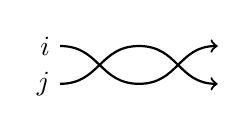
\begin{tikzpicture}[yscale=0.6, baseline=(x.base)]
        \node (x) at (0,0) {\vphantom{x}};

        \draw[thick, ->] (0,0.4) node[left] {$i$} to[out=0, in=180] (1,-0.4) to [out=0, in=180] (2,0.4);
        \draw[thick, ->] (0,-0.4) node[left] {$j$} to[out=0, in=180] (1,0.4) to [out=0, in=180] (2,-0.4);

    \end{tikzpicture}
  \ =
    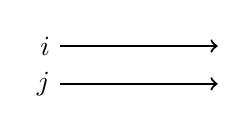
\begin{tikzpicture}[yscale=0.6, baseline=(x.base)]
        \node (x) at (0,0) {\vphantom{x}};

        \draw[thick, ->] (0,0.4) node[left] {$i$} -- (2,0.4);
        \draw[thick, ->] (0,-0.4) node[left] {$j$} -- (2,-0.4);

    \end{tikzpicture}
\end{equation}
\begin{equation}
    \Longleftrightarrow ~ R_{ji}(u_{j},u_{i})R_{ij}(u_{i},u_{j})  =  \mathrm{id}_{V_{i}\otimes V_{j}},
\end{equation}
and the Yang-Baxter equation
\begin{equation}
    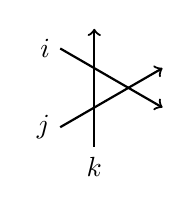
\begin{tikzpicture}[scale=0.5, baseline=(x.base)]
        \node (x) at (30:2) {};

        \draw[thick, ->] (0,0) node[left] {$j$} -- ++(30:3);
        \draw[thick, ->] (0,2) node[left] {$i$} -- ++(-30:3);
        \draw[thick, ->] (-30:1) node[below] {$k$} -- ++(0,3);

    \end{tikzpicture}
  \ =
    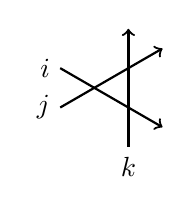
\begin{tikzpicture}[scale=0.5, baseline=(x.base)]
        \node (x) at (30:1) {};

        \draw[thick, ->] (0,0) node[left] {$j$} -- ++(30:3);
        \draw[thick, ->] (0,1) node[left] {$i$} -- ++(-30:3);
        \draw[thick, ->] (-30:2) node[below] {$k$} -- ++(0,3);

    \end{tikzpicture}
\end{equation}
\begin{equation}
  \Longleftrightarrow ~ R_{ij}(u_{i},u_{j})R_{ik}(u_{i},u_{k})R_{jk}(u_{j},u_{k})
    =  R_{jk}(u_{j},u_{k})R_{ik}(u_{i},u_{k})R_{ij}(u_{i},u_{j})
    ~ ,
\end{equation}
where the R-matrix $R_{ij}$ acts on $V_{i}\otimes V_{j}$ as an
intertwiner and trivial on $V_{k}$, etc. From these two relations
we can reproduce the commutativity of the transfer matrix. We should
emphasize that the Yang-Baxter equation is a local condition. When
the Boltzmann weight locally satisfies the Yang-Baxter equation, it
extends to the commutativity of the transfer matrix and hence to the
integrability of the model. In this sense, the Yang-Baxter equation
is the fundamental condition of integrability of a lattice model.


%No need to introduce Sigma?
Before getting into the discussion of brane construction, we would like
to generalize the above arguments to further higher-dimensional situations.
First of all, replace the two-torus $T^{2}$ with a general two-dimensional
surface $\Sigma$, along which line operators are wrapped. We now
have $S\times\Sigma$, and similarly to the above a lattice model
is defined on $\Sigma$ by line operators with spectral parameters.
Let us consider the case that we really have more extra dimensions
and a higher-dimensional theory is formulated on $S\times M\times\Sigma$,%
\footnote{Manifolds $M,\, N$ in this subsection are not necessarily the same as ones appeared in
previous subsections.}
%
where $M$ is some smooth manifold. In such a case, the line operators we had may
descend from extended operators of dimension greater than one. Let
$\mathsf{T}$ again be the new higher-dimensional theory, and suppose
that it is topological on $\Sigma$ and has extended operators $\mathcal{E}_{i}$
whose codimension is greater than $\dim S$. Place $\mathcal{E}_{i}$
on submanifolds of the form $\{ u_{i}\} \times N_{i}\times C_{i}$.
Since $\mathsf{T}[S\times M]$ is again regarded as a two-dimensional
TQFT defined on $\Sigma$, the correlation function of the operators
$\mathcal{E}_{i}$ in the full theory $\mathsf{T}$ still should coincide with the partition function
of an integrable lattice model $\mathsf{L}\big(\mathsf{T}[S\times M]\big)$.
The model is now defined on the lattice formed by the line operators
$\mathcal{E}_{i}\big(u_{i}; N_{i}\big)[C_i]$ winding along one-cycles $C_i$ on $\Sigma$,
which are the image of $\mathcal{E}_{i}$ in the two-dimensional theory
$\mathsf{T}[S\times M]$.

As well as we can view the higher-dimensional theory as a two-dimensional
TQFT, we may also view it as a theory $\mathsf{T}[\Sigma]$,
which is a QFT on $S\times M$ specified by the surface $\Sigma$.
In this theory, the operators $\mathcal{E}_{i}$ are seen as extended
operators $\mathcal{E}_{i}\big(C_{i}\big)$ supported on $\left\{ u_{i}\right\} \times N_{i}$.
Then, we have another relation
\begin{equation}
  \left\langle
    \prod_{i=1}^{l} \mathcal{E}_{i}\big(C_{i}\big)
    \big[\left\{ u_{i}\right\} \times N_{i}\big]
      \right\rangle_{\mathsf{T}\left[\Sigma\right],S\times M}
    =
      Z_{\mathsf{L}(\mathsf{T}[S\times M])}
        \big(\left\{ \mathcal{E}_{i}\big(u_{i}; N_{i}\big)[C_i]\right\})
    .
  \label{eq:correspondence_0}
\end{equation}
Thus, we finally arrive at a correspondence between a QFT on $S\times M$
equipped with extended operators and an integrable lattice model on
$\Sigma$.





\subsubsection{Brane construction and correspondence}

We have seen above that a lattice model is realized by a lattice of
line operators in a two-dimensional TQFT, and it is integrable if
the TQFT is embedded in higher dimensions and the line operators come
from extended operators localized in some directions of the extra
dimensions. Now we are ready to explain how to get such structures of correspondence
\eqref{eq:correspondence_0} using branes in string theory. The brane construction
here is still rather abstract. A little bit more concrete setups will
be given in next section. The reader may skip this subsection for
the first reading and jump to the next section.

Consider a type II string theory in a ten-dimensional spacetime
\begin{equation}
  \mathbb{R}^{4}  \times  T^{*}\Sigma  \times  \mathbb{R}^{2},
\end{equation}
where $\Sigma$ is a two-dimensional surface embedded in $T^{*}\Sigma$
as a zero section. Introduce a stack of $N$ NS5-branes supported
on $\mathbb{R}^{4}\times\Sigma\times \{ 0\} $ in this spacetime,
and D$p$-branes D$p_{i}$ on $\mathbb{R}^{p-1}\times\Sigma_{i}\times \{ 0\} $
ending on the NS5-branes, where $\mathbb{R}^{p-1}$ is a subspace
of $\mathbb{R}^{4}$ (assuming $p\leq5$) and $\Sigma_{i}$ are surfaces
in $T^{*}\Sigma$ such that $\Sigma_{i}\cap\Sigma=C_{i}$; see figure \ref{fig:Dp_on_NS5}.
Provided that $\Sigma_{i}$ are suitably chosen, this brane system
preserves four supercharges.


%FIGURE
\begin{figure}
  \centering

    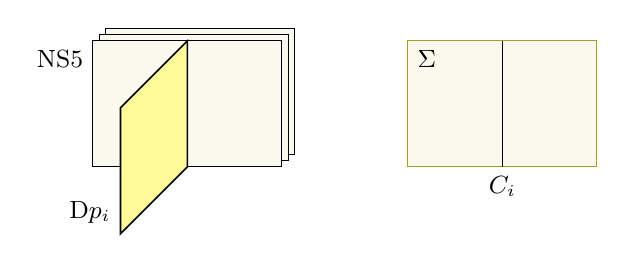
\begin{tikzpicture}[scale=0.8]    %, baseline=(x.base)]        \node (x) at (0,0) {\vphantom{x}};

        \filldraw[fill=olive!5, xshift=0.2cm, yshift=0.2cm] (0,0) rectangle (-3,2);
        \filldraw[fill=olive!5, xshift=0.1cm, yshift=0.1cm] (0,0) rectangle (-3,2);
        \filldraw[fill=olive!5] (0,0) rectangle (-3,2) node[below left] {\small NS5};

        \filldraw[semithick, fill=yellow!40] (-1.5,0) -- ++(0,2) -- ++(225:1.5) -- ++(0,-2) node[above left] {\small D$p_{i}$} -- cycle;

        \filldraw[color=olive!80, fill=olive!5] (2,2) node[color=black, below right] {\small $\Sigma$} rectangle (5,0);
        \draw[semithick] (3.5,0) node[below] {\small $C_i$} -- ++(0,2);

    \end{tikzpicture}

  \caption{The D$p$-brane D$p_i$ ending on the NS5-branes creates a defect $\mathcal{E}_{\rm{D}p_i}$ along $C_i$.}
  \label{fig:Dp_on_NS5}
\end{figure}


The low-energy dynamics of the NS5-branes is governed by a six-dimensional
theory $\mathsf{T}_{\mathrm{NS5}}$ on $\mathbb{R}^{4}\times\Sigma$.
The theory $\mathsf{T}_{\mathrm{NS5}}$ is depending on whether IIA
or IIB theory we are considering:
\begin{align*}
  \textrm{IIA : }  &  \mathcal{N} = (2,0)  \text{ superconformal QFT of type } A_{N-1},  \\
  \textrm{IIB : }  &  \mathcal{N} = (1,1)  \text{ super Yang-Mills theory with gauge group } \SU(N).
\end{align*}
The theory $\mathsf{T}_{\mathrm{NS5}}$ is formulated on $\mathbb{R}^{4}\times\Sigma$,
with topological twist along $\Sigma$ which breaks half of sixteen
supercharges. In this twisted theory, D$p_{i}$ create $p$-dimensional
defects $\mathcal{E}_{\mathrm{D}p_{i}}$ on $\mathbb{R}^{p-1}\times C_{i}$,
reducing the number of unbroken supercharges to four. From the point
of view of a four-dimensional observer, this brane configuration gives
half-BPS defects $\mathcal{E}_{\mathrm{D}p_{i}}(C_{i})$
in an $\mathcal{N}=2$ theory $\mathsf{T}_{\mathrm{NS5}}[\Sigma]$.
The total system is invariant under a $\U(1)$ R-symmetry originating
from the rotational symmetry on the $\mathbb{R}^{2}$ factor of the
ten-dimensional spacetime.

Let us take a three-manifold $M$ and $(p-2)$-submanifolds $N_{i}$
of $M$, and modify the above construction so that the world-volumes
of the NS5-branes and the D$p$-branes become $S^{1}\times M\times\Sigma$
and $S^{1}\times N_{i}\times\Sigma_{i}$, respectively. At low energies,
we get the same theory $\mathsf{T}_{\mathrm{NS5}}$ formulated on
$S^{1}\times M\times\Sigma$ and defects $\mathcal{E}_{\mathrm{D}p_{i}}$
located on $S^{1}\times N_{i}\times C_{i}$. In general, this modification
completely breaks supersymmetry. For certain choices of $M$ and $N_{i}$,
however, there is a string background in which a fraction of supersymmetry
is still preserved. In such a background, the path integral computes
the twisted partition function, or \emph{supersymmetric index} of $\mathsf{T}_{\mathrm{NS5}}$,
defined by a trace with respect to the Hilbert space on $M\times\Sigma$ in the presence
of defects $\mathcal{E}_{\mathrm{D}p_{i}}$ inserted on $N_{i}\times C_{i}$
(recall that for a closed manifold with thermal circle, QFT produces a number represented as a trace,
such as \eqref{eq:qm_number}).

A salient feature of supersymmetric indices is that they are protected
against continuous changes of various parameters of the theory. This
means that the index of our theory is invariant under deformations
of the geometric data of $\Sigma$ and $C_{i}$, such as the metric
on $\Sigma$ and the shapes of $C_{i}$. In other words, the theory
$\mathsf{T}_{\mathrm{NS5}}$ on $S^{1}\times M\times\Sigma$ is topological
on $\Sigma$, as far as the computation of the index is concerned.

To relate the present setup to the the previous situation \eqref{eq:correspondence_0},
we apply T-duality along the circle $S^{1}$. It turns D$p_{i}$
into D$(p-1)$-branes D$(p-1)_{i}$, localized
at points $u_{i}$ along the dual circle $\tilde{S}^{1}$, while sending
the NS5-branes to those in the other type II string theory. The new
NS5-branes produce the dual six-dimensional theory $\tilde{\mathsf{T}}_{\mathrm{NS5}}$
on $\tilde{S}^{1}\times M\times\Sigma$, and in this theory D$(p-1)_{i}$
create $(p-1)$-dimensional defects $\mathcal{E}_{\mathrm{D}(p-1)_{i}}$
on $\{ u_{i}\} \times N_{i}\times C_{i}$. Thus we are
in the situation studied before, and the correlation function of $\mathcal{E}_{\mathrm{D}(p-1)_{i}}$
for this configuration coincides with the partition function
of an integrable lattice model:
\begin{equation}
  \left\langle
    \prod_{i=1}^l \mathcal{E}_{\mathrm{D}p_i}(C_i) \big[S^1 \times N_i\big]
      \right\rangle_{\mathsf{T}_{\mathrm{NS5}}[\Sigma],S^{1}\times M}
    =
      Z_{\mathsf{L}\big(\tilde{\mathsf{T}}_{\mathrm{NS5}}\big[\tilde{S}^{1}\times M\big]\big)}
      \big( \left\{ \mathcal{E}_{\mathrm{D}(p-1)_i} \big(u_i; N_i\big) [C_i]\right\} \big).
\end{equation}
Here the left-hand side is expressed in the original frame; it implicitly
depends on each spectral parameter $u_{i}$ through the holonomy $\exp(2\pi\mathrm{i}u_{i})$
around $S^{1}$ of the gauge field for the flavor symmetry U$(1)_{i}$
supported on D$p_{i}$. The holonomy appears in the index as a refinement
parameter, or called \emph{fugacity}, associated with $\U(1)_i$.





\subsubsection{Defects as transfer matrices}
\label{sec:defects}

Finally, we apply the construction developed so far
to the main theme of this paper: integrable lattice models and defects
as transfer matrices. Let us consider the brane construction for $p=5$ case.
To conform with the standard convention, take
S-duality first and we still have D5- and NS5-branes
\begin{align*}
  N  \,  \mathrm{D5}   &  \quad S^{1}  \times  M  \times  \Sigma,  \\
  \mathrm{NS5}_{i}    &  \quad S^{1}  \times  N_{i}  \times  \Sigma_{i},
\end{align*}
where NS$5_{i}$ create defects $\mathcal{E}_{\mathrm{NS}5_{i}}$
on $S^{1}\times N_{i}\times C_{i}$.

One should notice that in this setup we necessarily have $N_{i}=M$
and thus the defects $\mathcal{E}_{\mathrm{NS}5_{i}}$ fill the whole
$S^{1}\times M$, which produces a four-dimensional theory
\begin{equation*}
  \mathsf{T}_{\mathrm{D5NS5}}[\Sigma]
\end{equation*}
with $\mathcal{N}=1$ supersymmetry. Then we now have
\begin{equation}
  \left\langle  1  \right\rangle_{\mathsf{T}_{\mathrm{D5NS5}}[\Sigma], S^{1}\times M}
    =Z_{\mathsf{L}\big(\mathsf{T}_{\mathrm{D5NS5}}[S^{1}\times M]\big)}
      \big( \left\{ \mathcal{E}_{i}(S^{1}\times M) [C_i]\right\} \big).
\end{equation}
For example, when $M=S^{3}$, the left-hand side is given by the supersymmetric
index for $\mathcal{N}=1$ theory and the right-hand side corresponds
to the partition function of Bazhanov-Sergeev integrable lattice model
\cite{Bazhanov:2010kz,Bazhanov:2011mz,Spiridonov:2010em,Yamazaki:2012cp}. When $M=L(p,1)$,
lens space, the left-hand side is computed in \cite{Yamazaki:2013nra}, which
defines a new integrable lattice model through this correspondence.

The brane tiling construction of integrable lattice models can be
enriched by introducing additional defects. Besides the previously
defined D5NS5-brane system, let us consider a D3-brane such as
\begin{align}
  \mathrm{D3}    &  \quad S^{1}  \times  N  \times  C  \times  \mathbb{R}_{+}, \label{eq:D3}\\
  \mathrm{D3'}   &  \quad S^{1}  \times \{ 0\}  \times  C'  \times  \mathbb{R}^{2}, \label{eq:D3'}
\end{align}
where $N$ is a curve in $M$ and $C,\,C'$ are one-cycles on $\Sigma$.
These D3-branes create new extended defect operators elongated in $S^1\times N$ and $S^1$, respectively.
A single D3-brane insertion corresponds to a new oriented line $C,\,C'$ in
the integrable lattice model, which we represent by a dashed line.
Now that we have two kinds of lines originating from five-branes and a D3-brane,
we can define three kinds of R-matrices:
\begin{equation}
  R=
    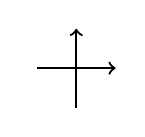
\begin{tikzpicture}[scale=0.5, baseline=(x.base)]
        \node (x) at (0,0) {\vphantom{x}};

        \draw[thick, ->] (0,0) -- (2,0);
        \draw[thick, ->] (1,-1) -- (1,1);

    \end{tikzpicture}
  ~ ,
  \quad
  L=
    \begin{tikzpicture}[scale=0.5, baseline=(x.base)]
        \node (x) at (0,0) {\vphantom{x}};

        \draw[thick, densely dashed, ->] (0,0) -- (2,0);
        \draw[thick, ->] (1,-1) -- (1,1);

    \end{tikzpicture}
  ~ ,
  \quad
  \mathcal{R}=
    \begin{tikzpicture}[scale=0.5, baseline=(x.base)]
        \node (x) at (0,0) {\vphantom{x}};

        \draw[thick, densely dashed, ->] (0,0) -- (2,0);
        \draw[thick, densely dashed, ->] (1,-1) -- (1,1);

    \end{tikzpicture}
  ~ .
\end{equation}
The middle one is usually called \emph{L-operator}. Correspondingly,
we have four Yang-Baxter equations, involving zero to three dashed
lines. Those that involving one or two dashed line,
\begin{equation}
    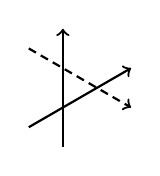
\begin{tikzpicture}[scale=0.5, baseline=(x.base)]
        \node (x) at (30:2) {};

        \draw[thick, ->] (0,0) -- ++(30:3);
        \draw[thick, densely dashed, ->] (0,2) -- ++(-30:3);
        \draw[thick, ->] (-30:1) -- ++(0,3);

    \end{tikzpicture}
  \ = \
    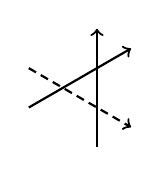
\begin{tikzpicture}[scale=0.5, baseline=(x.base)]
        \node (x) at (30:1) {};

        \draw[thick, ->] (0,0) -- ++(30:3);
        \draw[thick, densely dashed, ->] (0,1) -- ++(-30:3);
        \draw[thick, ->] (-30:2) -- ++(0,3);

    \end{tikzpicture}
%
  \quad  \text{and}  \quad
%
    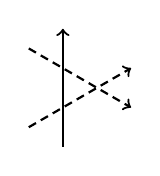
\begin{tikzpicture}[scale=0.5, baseline=(x.base)]
        \node (x) at (30:2) {};

        \draw[thick, densely dashed, ->] (0,0) -- ++(30:3);
        \draw[thick, densely dashed, ->] (0,2) -- ++(-30:3);
        \draw[thick, ->] (-30:1) -- ++(0,3);

    \end{tikzpicture}
  \ = \
    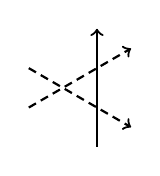
\begin{tikzpicture}[scale=0.5, , baseline=(x.base)]
        \node (x) at (30:1) {};

        \draw[thick, densely dashed, ->] (0,0) -- ++(30:3);
        \draw[thick, densely dashed, ->] (0,1) -- ++(-30:3);
        \draw[thick, ->] (-30:2) -- ++(0,3);

    \end{tikzpicture}
\end{equation}
are called \emph{RLL relations}. The effect of the insertion of such
an additional defect on the lattice model is seen in terms of the
L-operator. The neighborhood of the dashed line looks like
\begin{equation}
    \begin{tikzpicture}[scale=0.9, baseline=(x.base)]
        \node (x) at (0,0) {\vphantom{x}};

        \draw[thick, ->] (0.3,-0.4) -- (0.3, 0.6);
        \draw[thick, ->] (0.9,-0.4) -- (0.9, 0.6);
        \draw[thick, ->] (2.7,-0.4) -- (2.7, 0.6);

        \draw[thick] (0,0) arc (270:90:0.1);
        \draw[thick, ->-=0.24, densely dashed] (0,0) -- (3,0);
        \draw[thick] (3,0) arc (-90:90:0.1);

        \draw[preaction={draw=white, ultra thick}, thick, loosely dotted] (1.4,0) -- (2.1,0);

    \end{tikzpicture}
    \quad .
\end{equation}
This diagram shows that the defect acts on the lattice model by a
transfer matrix constructed from L-operators. Thus, the insertion
of a defect operator in four-dimensional theory represented by
\eqref{eq:D3} or \eqref{eq:D3'} is mapped into lattice
model side as the action of a transfer matrix constructed from L-operators.

What we will discuss in detail in the subsequent sections
are the introduction of a single D3-brane \eqref{eq:D3} and \eqref{eq:D3'} to the
D5NS5-brane system, and investigate the correspondence between supersymmetric gauge theories
and integrable lattice models with the additional
defects. In the next two sections, we are exploring the followings:
\begin{enumerate}
	\item For the case of single D3 \eqref{eq:D3}, let $M=S^{3}$, $\Sigma=T^{2}$, and $N=S^{1}$.
Then the D3 creates a surface defect on $S^{1}\times S^{1} \subset S^1\times S^3$ and it
acts on the supersymmetric index as a transfer matrix in the corresponding
lattice model:
\begin{align}
  \left\langle  1  \right\rangle_{\mathsf{T}_{\mathrm{D5NS5}}[\Sigma],S^{1}\times S^{3}}
    &  =  \mathcal{I}_{S^{1}\times S^{3}}(p,q,t),\\
  Z_{\mathsf{L}\big(\mathsf{T}_{\mathrm{D5NS5}}[S^{1}\times S^{3}]\big)}
    \big( \left\{ \mathcal{E}_{i}(S^{1}\times S^{3})[C_i]\right\} \big)
    &  =  Z_{\mathrm{Bazhanov-Sergeev}},
\end{align}
the surface defect index is represented as a difference operator
acting on the original supersymmetric index \cite{Gaiotto:2012xa,Gadde:2013dda},
\begin{equation}
  \left\langle S_{(r,s)}\right\rangle_{\mathsf{T}_{\mathrm{D5NS5}}[\Sigma]}
    =
      \mathfrak{S}_{(r,s)} \, \mathcal{I}_{S^{1}\times S^{3}}(p,q,t).
\end{equation}
\item For the case of single D3$'$ \eqref{eq:D3'}, let $M=\mathbb{R}^{3}$ and $\Sigma=T^{2}$.
D3$'$ creates a line defect wrapping the thermal circle $S^{1}$ and it acts on the quantum
Hilbert space of a spin chain as a transfer matrix, since now we have
non-compact three-manifold $\mathbb{R}^{3}$.
This spin chain has a equivalent lattice model description, and it is really an integrable model of
trigonometric type. The line defect in the
four-dimensional theory is realized as a Wilson-'t Hooft line operator
$T$, and its magnetic charge and electric charge $(\mathbf{m},\mathbf{e})$
is specified by the one-cycle $C'$ winding around the torus $T^{2}$. As it
turns out, the vacuum expectation values (vevs) of Wilson-'t Hooft
lines realize the deformation quantization of the Hitchin moduli space,
and are naturally quantized by the Weyl quantization:
\begin{equation}
  \textrm{Weyl quantization of }  \left\langle  T_{\left(\mathbf{m},\mathbf{e}\right)}  \right\rangle
  =  \textrm{trigonometric transfer matrix.}
\end{equation}
\end{enumerate}
%

{\bf In the following subsections, we study these correspondences.
Sections 3 \& 4 are almost independent.}





%\subsection{xxx}









%%%%%%%%%%%%%%%%%%%%%%%%%%%%%%%%%%%%%%%%%%%%%%%%%%%%%%%%%



\bibliographystyle{Common/utphys}
%\nocite{*}
\bibliography{Common/Ref}



\end{document}